% Multi-Survey Spectral Anomaly Detection
% Houston Golden — 2026
% arXiv submission: astro-ph.IM / astro-ph.GA / astro-ph.CO
%
% Compile: pdflatex paper3_draft && bibtex paper3_draft && pdflatex paper3_draft && pdflatex paper3_draft

\documentclass[aps,prd,twocolumn,superscriptaddress,showpacs,preprintnumbers,nofootinbib,longbibliography,floatfix]{revtex4-2}

\usepackage{amsmath,amssymb,amsfonts}
\usepackage{graphicx}
\usepackage{bm}
\usepackage{hyperref}
\usepackage{xcolor}
\usepackage{booktabs}
\usepackage{multirow}
\usepackage{dcolumn}
\usepackage{enumitem}
\usepackage{mathtools}
\usepackage[utf8]{inputenc}

\hypersetup{
  colorlinks=true,
  linkcolor=blue!60!black,
  citecolor=blue!60!black,
  urlcolor=blue!60!black
}

% Custom commands
\newcommand{\fnl}{f_{\rm NL}}
\newcommand{\sigfnl}{\sigma(f_{\rm NL})}
\newcommand{\ie}{i.e.}
\newcommand{\eg}{e.g.}
\newcommand{\cf}{cf.}
\newcommand{\etal}{\textit{et~al.}}
\newcommand{\BigAE}{\textsc{BigAE}}
\newcommand{\Neff}{N_{\rm eff}}
\newcommand{\Mpc}{\,\text{Mpc}}

\begin{document}

%\preprint{arXiv:XXXX.XXXXX}

\title{Spectrally Unusual Sources at Scale: A Multi-Survey Catalog of\\
378{,}280 Path-C Unique Anomalies and\\
Native-Trained Novelty Fractions from 37.3 Million Sources and Map Patches}

\author{Houston Golden}
\email{houston@hubify.com}
\affiliation{Independent Researcher, Los Angeles, California, USA}

\date{June 2026}
% v3.1.75 (2026-06-05, aggressive condensation 32pp → 20pp. Abstract 2.5pp→0.8pp;
%   intro para 4 compressed; training in-sample validation 7kch→1.3kch; f_NL
%   section 16kch→3.1kch; NANOGrav 6.7kch→1.5kch; Limitations 4.9kch→1.6kch;
%   conclusions 8.6kch→2.7kch; App E PTA MCMC 6.4kch→2.1kch; Path-C enumerate
%   6.1kch→2.0kch; data-availability 2.9kch→0.7kch. Zero errors, zero Overfull.
%   All headline numbers preserved: 378,280 / 37.3M / 378,080 / 200 / 17.8% / 7.9%.)
% v3.1.74 (2026-06-05, structural condensation: trimmed version-history preamble,
%   condensed per-survey prose, compressed Path-C caveats to table, replaced
%   App D single-family galleries (figs a2-a10) with companion-repo pointer,
%   tightened abstract second paragraph and intro second/third paragraphs).
%   No scientific content changed; all headline numbers preserved.
% v3.1.73 (2026-06-03, R9-triage bib-hygiene polish PER-M1/PER-m1/PER-m2/PER-n1).
%   Added 4 bib entries (Yoo+2009 arXiv:0907.0707, Bonvin\&Durrer 2011 arXiv:1105.5280,
%   Challinor\&Lewis 2011 arXiv:1105.5292, DiDio+2013 arXiv:1307.1459) and converted
%   §pathc_caveats(e) prose mentions to explicit \cite{} commands. Added arXiv:0903.0631
%   to Cai:2009fn entry. Expanded Foreman-Mackey entry to full Publ.\ Astron.\ Soc.\ Pac.
%   format with page range. Standardized Heinrich2023 entry to spell out JCAP +
%   publication-year note (bibkey retained for arXiv-submission-year continuity).
%   No content changes. Polish-tier only.
% v3.1.71 (2026-06-01, cross-vendor R-round 2026-06-01_R-multi-true95 closure on v3.1.70).
%   Three direct-vendor reviews (Grok-4, GPT-4o, Perplexity Sonar Pro) returned 0 VERIFIED
%   findings — all 13 findings classified STALE/FALSIFIED/OPINION. §pathc_caveats (a)-(j)
%   all CLOSED. Deliverable: synthesis MD + version bump + PDF mirror + Convex bump.
%
% [Earlier version history (v3.1.40–v3.1.70) archived in
%  project-context/peer-reviews/version-history-archive.md]

\begin{abstract}
We present the largest-scale application of autoencoder anomaly detection across seven astronomical archives, applying the \BigAE{} autoencoder framework to 37.3~million sources and CMB map patches (DESI~DR1, SDSS~DR18, LAMOST~DR10, eROSITA~DR1, Planck, Gaia~DR3, NEOWISE; ACT~DR6 quarantined as a cross-transfer artifact). After per-survey native retraining and $7$-way positional deduplication at $5''$, the catalog contains $\mathbf{378{,}280}$ unique anomalies: $\mathbf{378{,}080}$ point-source object detections from six photometric/spectroscopic surveys plus $\mathbf{200}$ Planck CMB map-patch sky regions. Downstream object-level analyses (SIMBAD/NED cross-matching, multi-tracer $f_{\rm NL}$ selection) should use the $\mathbf{378{,}080}$ point-source tier; the recommended catalog-grade subset is $\sim\!265{,}000$ unique objects (DESI $+$ SDSS $+$ eROSITA $+$ Gaia $+$ NEOWISE), which excludes the LAMOST exploratory tier ($\sim\!113{,}000$ objects retained as a methodological lesson: 98\% blue-excess training-bias artifact, injection-recovery gate FAIL). The point-source tier is $\sim\!141\times$ the size of the largest prior single-survey anomaly catalog~\cite{Liang2023}; the DESI-only axis ($195{,}829$ anomalies) is a $\sim\!73\times$ like-for-like increase. Extended archival cross-matching of the top-$1{,}000$ DESI anomalies against 20 curated all-sky catalogs via CDS X-Match yields a genuine novelty fraction of $\sim\!17.8\%$ (single-sample point estimate at the top-$1{,}000$ score stratum; full-catalog rate empirically untested). A Path-C rebuild protocol resolves cross-transfer artifacts: $21.5\times$ LAMOST rate compression and $\sim\!6500\times$ SDSS rate compression after native retraining; DESI 5-fold Jaccard stability $\bar{J} = 0.862$ ($\geq 0.70$ gate, PASS). Six injection-recovery gates: 3 PASS (SDSS 64\%, Planck 100\%, NEOWISE 100\%) and 3 FAIL-with-diagnostic at $5\sigma$ (LAMOST 5.8\%, Gaia 5.2\%, eROSITA 1.2\%; eROSITA cross-validation stability 81.5\%). Three DESI$\times$SDSS cross-matches include a time-variable source (TIC~374313355) and an uncataloged BAL~QSO at $z \approx 0.86$. An empirical Landy--Szalay bias measurement on the $5{,}384$ QSO-candidate sample yields $\alpha_{\rm jk} = 0.19 \pm 0.65$ ($<\!1\sigma$ from null); inserting this into the Fisher-positivity-respecting form $1/\sigfnl^2 = F_0 + c\,\alpha^2$ gives a central forecast $\sigfnl = 8.14$ with $1\sigma$ envelope $[3.92, 8.98]$ (7.9\% improvement consistent with no improvement at $<\!1\sigma$; $\sigfnl^{\rm std} = 8.98$ single-tracer baseline). A NANOGrav 15-yr KDE free-spectrum MCMC yields $\gamma = 2.567 \pm 0.382$; the matter-bounce prediction $\gamma = 3.0$ sits at $+1.13\sigma$ (marginally consistent) and SMBHB $\gamma = 4.33$ at $+4.61\sigma$ (Savage-Dickey $B_{\rm MB/SMBHB} = 7.1\!\times\!10^3$). The catalog, model weights, and reproducibility scripts are publicly released.
\end{abstract}

\keywords{anomaly detection, machine learning, spectroscopic surveys, multi-survey catalogs, autoencoder}

\maketitle


%% ============================================================
%%  1. INTRODUCTION
%% ============================================================
\section{Introduction}\label{sec:intro}

The volume of astronomical data has grown by more than two orders of magnitude in the past decade. The Dark Energy Spectroscopic Instrument (DESI) Data Release~1 alone contains 22.5 million spectra~\cite{DESI2025DR1}, LAMOST DR10 contributes 11.4 million~\cite{LAMOST_DR10}, and the Sloan Digital Sky Survey DR18 provides 2.3 million spectroscopically characterized objects~\cite{SDSS_DR18}. When combined with multi-wavelength catalogs from eROSITA~\cite{eROSITA_DR1}, Gaia~\cite{GaiaDR3}, NEOWISE~\cite{NEOWISE}, and microwave sky surveys from Planck~\cite{Planck2018} and ACT~\cite{ACT_DR6}, the total data volume accessible to a single research group now exceeds tens of millions of sources across the electromagnetic spectrum.

Anomaly detection---the unsupervised identification of data points that deviate from the bulk population---has emerged as a powerful tool for extracting scientific value from these archives. Baron \& Poznanski~\cite{Baron2017} demonstrated autoencoder anomaly detection on SDSS spectra, finding unusual white dwarfs and cataclysmic variables. Liang \etal~\cite{Liang2023} applied a normalizing-flow autoencoder to $\sim\!250{,}000$ DESI EDR spectra, finding 2{,}685 anomalies (1.07\%). Nicolaou \etal~\cite{Nicolaou2026} extended this with the Astronomaly active-learning framework on 208{,}000 EDR spectra. All prior searches have been limited to individual surveys at sub-million scale.

We are motivated by two scientific goals. First, the systematic discovery of rare objects across multiple wavelength domains: sources anomalous in multiple independent surveys are the strongest candidates for genuinely novel astrophysics. Second, the quasi-matter bounce model predicts $\fnl = -35/8 = -4.375$~\cite{Wands2010,Cai:2009fn,WilsonEwing2012}, testable at $3$--$5\sigma$ with SPHEREx~\cite{SPHEREx2014} under the multi-tracer methodology of Heinrich \etal~\cite{Heinrich2023} ($\sigfnl \approx 0.7$ bispectrum-only forecast). Anomaly-detected high-redshift QSO candidates represent a previously unexploited high-bias tracer reservoir that can tighten $\fnl$ constraints via the multi-tracer technique~\cite{Seljak2009,Hamaus2012}.

In this work we apply the \BigAE{} autoencoder framework to seven retained archives (DESI~DR1, SDSS~DR18, LAMOST~DR10, eROSITA~DR1, Planck CMB, Gaia~DR3, NEOWISE; catalog counts appear as $378{,}080 + 200 = 378{,}280$ throughout to distinguish point-source detections from CMB map-patch sky-regions). A first-pass cross-transfer scan exposed two failure modes---98\% LAMOST blue-excess from training drift and an undertrained CMB autoencoder---motivating the Path-C native-retrain rebuild (\S\ref{sec:pathc}). Sections~\ref{sec:method}--\ref{sec:pathc} describe the method; \S\ref{sec:surveys} reports survey-by-survey results; \S\ref{sec:crosssurvey} cross-survey analysis; \S\ref{sec:fnl} cosmological applications; \S\ref{sec:discussion} limitations and conclusions.


%% ============================================================
%%  2. METHOD
%% ============================================================
\section{Method}\label{sec:method}

\subsection{\BigAE{} Architecture}\label{sec:architecture}

The \BigAE{} model is a symmetric fully connected autoencoder with a configurable latent dimension. The architecture is adapted per survey to match the dimensionality of the input feature space: for spectroscopic surveys (DESI, SDSS, LAMOST), the input dimension is 496 (three-arm spectra downsampled by a factor of 16 from the native resolution); for photometric and catalog surveys (eROSITA, Gaia, NEOWISE), the input dimension matches the number of catalog features (47, 20, and 15, respectively); and for CMB surveys (Planck, ACT), the input is a $64 \times 64$ pixel patch flattened to 4{,}096 features.

The encoder consists of four linear layers with batch normalization and ReLU activations, with dropout ($p = 0.15$, $0.10$) after the first two layers; the decoder mirrors the encoder. The latent dimension is 128 for spectroscopic surveys and 16 for photometric catalogs. The Path-C native CMB convolutional autoencoder (Planck; \S\ref{sec:planck}) uses three convolutional layers $+$ a 128-dim fully connected bottleneck ($1.1\!\times\!10^6$ parameters). Total parameter count: ${\sim}120{,}000$ (photometric) to $660{,}000$ (spectroscopic); architecture shown schematically in Fig.~\ref{fig:architecture}. \BigAE{} is a deterministic autoencoder (not variational), prioritizing reconstruction fidelity and anomaly-score interpretability.

\subsection{Training and Scoring}\label{sec:training}

For each survey, the model is trained on a representative subset of the data (47{,}000 spectra for DESI, proportionally sampled subsets for other surveys) using the Adam optimizer with initial learning rate $10^{-3}$, batch size 512, and ReduceLROnPlateau scheduling (patience 5, factor 0.5), minimizing per-element mean-squared error (MSE). Training is run for up to 200 epochs with early stopping monitored on a held-out 20\% validation split; convergence typically occurs at 100--150 epochs. (The native CMB convolutional autoencoder uses a different schedule---see Section~\ref{sec:planck}---and individual native retrains may differ in patience settings as noted in the survey-specific sections.)

The raw per-element mean-squared reconstruction error between input and reconstruction is
\begin{equation}\label{eq:score_raw}
\mathrm{MSE}(\mathbf{x}) = \frac{1}{N}\sum_{i=1}^{N}(x_i - \hat{x}_i)^2,
\end{equation}
where $\hat{\mathbf{x}} = \BigAE(\mathbf{x})$ and $N$ is the input dimensionality.

\paragraph{Canonical anomaly score $S$ (one definition for the whole paper).}
\emph{Throughout this paper, ``$S$'' refers without exception to the per-survey standardized (``$z$-scored'' in the statistical sense) reconstruction residual (note: `$z$-scored' here is the statistics term for a mean-subtracted, variance-normalized quantity; spectroscopic redshift is always written $z$ with astrophysical context; the anomaly score $S$ is never called `$z$' in this paper to avoid ambiguity)}
\begin{equation}\label{eq:score}
S(\mathbf{x}) \;\equiv\; \frac{\mathrm{MSE}(\mathbf{x}) - \mu_{\rm val}}{\sigma_{\rm val}},
\end{equation}
where $\mu_{\rm val}$ and $\sigma_{\rm val}$ are the mean and standard deviation of $\mathrm{MSE}$ on the held-out 20\% validation split of that survey's training pool. $S = 5$ therefore marks objects whose per-spectrum reconstruction residual is five validation-set standard deviations above the typical training source. For DESI~DR1, $\mu_{\rm val} \!\approx\! 0.0287$ (validation MSE) and $\sigma_{\rm val}$ is set such that the $S>5$ catalog threshold corresponds to $\mathrm{MSE} \!\approx\! 0.143$ on the rescaled scale. For spectroscopic surveys, we additionally decompose the score into per-band contributions $r_B$, $r_R$, $r_Z$ computed over the blue (3600--6200~\AA), red (6200--8200~\AA), and near-infrared (8200--9800~\AA) subsets (Fig.~\ref{fig:example_spectra}).

Two threshold families are in use (summarized in Table~\ref{tab:survey_summary} footnotes): DESI~DR1 and SDSS~DR18 use an absolute canonical-$S$ cut at $S > 5.0$ (corresponding to a fixed reconstruction-MSE threshold anchored by each survey's $(\mu_{\rm val}, \sigma_{\rm val})$); LAMOST~DR10 and Gaia~DR3 use the 99th-percentile of the per-survey $S$ distribution; eROSITA uses a data-driven IsolationForest score-knee threshold; Planck and NEOWISE use a fixed top-1\% selection. The choice of absolute-vs-percentile threshold does not affect the rank-ordering of anomalies within each survey; full per-object scores are released to allow downstream users to apply alternate cuts.

\paragraph{In-sample scoring and held-out validation.}
The DESI~DR1 anomaly catalog is scored on the full 22.5~million-spectrum set, which includes the 47{,}000 training spectra. Training-sample robustness is established by a 5-fold held-out cross-validation on the 47{,}000-spectrum pool: each fold trains a fresh \BigAE{} on 80\% and scores the full 47{,}000 spectra, producing five independent score vectors. Mean pairwise Jaccard overlap of each fold's top-$1\%$ anomaly set is $\bar{J} = 0.862$ (minimum $0.777$; gate $\geq 0.70$, PASS). Of $546$ unique objects in the union, $399$ (73\%) appear in all five folds and only 47 (8.6\%) are single-fold singletons; details in \S\ref{sec:pathc_caveats}~(i). An independent OOD validation on 100k unseen DESI spectra retrieved via NOIRLab SPARCL (seed distinct from the training pool) confirms that in-sample and out-of-sample anomaly rankings are consistent; the production-vs-5-seed-control Jaccard is $\bar{J}_{\rm prod\times ctrl} = 0.732$ (gate $\geq 0.50$, PASS). The $S>5$ absolute MSE-anchored threshold applied to the full 22.5M curated catalog yields the $0.87\%$ anomaly rate; applying it to a random uncurated SPARCL sweep flags $>50\%$ of spectra (a catalog-curation effect, not a threshold artifact; see \S\ref{sec:pathc_caveats}~(b) for the full OOD reconciliation).

\subsection{GPU Inference Pipeline}\label{sec:inference}

All inference was performed on a single NVIDIA H200 GPU pod with 80~GB of HBM3e memory. Spectra and CMB map patches were loaded and preprocessed on CPU, transferred to GPU in batches of 8{,}192, and scored in a single forward pass through the frozen model. The total processing time across the seven retained surveys plus the quarantined ACT~DR6 cross-transfer scan (Appendix~\ref{sec:act_appendix}) was approximately 42 hours (wall-clock), dominated by the DESI DR1 scan (19{,}705~s for 22.5M spectra, throughput ${\sim}1{,}142$~spectra/s) and the LAMOST DR10 scan (11.4M spectra). The CMB and photometric surveys each required $< 10$~seconds of GPU time. Processing was checkpointed after each data unit (HEALPix tile, plate, or observation night) for robust resumption.


\subsection{Path-C Rebuild Methodology: Native Retrains as Core Protocol}\label{sec:pathc}

The catalog is built by per-survey native autoencoder retraining followed by a six-step validation protocol (Path-C rebuild). \emph{Native retrains are the core methodology:} each survey carries its own \BigAE{} trained on a quality-selected subset of that survey's own data; the published anomaly set is the top-percentile cut of the survey's own model applied to its own catalog. The initial cross-transfer scan (DESI-trained \BigAE{} applied to SDSS, LAMOST, and CMB) is preserved in Table~\ref{tab:survey_summary} and \S\ref{sec:lamost_lesson} as the before/after diagnostic that motivates the native-retrain methodology; it is not a science result.

The rebuild proceeds in six steps:
\begin{enumerate}[leftmargin=*]
  \item \textit{Native retrain (two-part gate).} A fresh \BigAE{} is trained on a $2$--$5\!\times\!10^5$-spectrum quality-selected subset of each survey's own data. Retained if (a)~validation loss $\leq 0.30$ after $\leq\!100$ epochs, \emph{or} (b)~injection-recovery $\geq\!50\%$ at $5\sigma$. SDSS gates PASS at val\_loss $0.0311$ (criterion a); LAMOST at $0.0329$ (a); Planck CMB native convolutional autoencoder at val\_loss $0.4437$ / $100\%$ injection-recovery (criterion b).
  \item \textit{Native CMB retrain.} A convolutional autoencoder (3 conv layers $+$ 128-dim FC bottleneck, $1.1\!\times\!10^6$ parameters) trained on $2\!\times\!10^5$ galactic-plane-masked ($|b|\geq 20^\circ$) SMICA patches supersedes the cross-transfer checkpoint.
  \item \textit{Full-survey re-score.} Each native-retrained model is applied to the full survey catalog in streaming batches; the same top-percentile cut from Table~\ref{tab:survey_summary} is re-applied.
  \item \textit{Systematics mask.} NEOWISE ecliptic-pole mask ($|b_{\rm ecl}|<80^\circ$) retains $419/436$ anomalies ($96.1\%$); the rejected $3.9\%$ polar-cap fraction is $2.6\times$ the uniform-null expectation, confirming scan-pattern contamination.
  \item \textit{Injection-and-recovery.} 500 planted signals per survey at six amplitude levels ($0.5$--$20\times\sigma$); recovery above the 99th-percentile clean-MSE threshold. Results: 3 PASS (SDSS 64\%, Planck 100\%, NEOWISE 100\%) and 3 FAIL-with-diagnostic (LAMOST 5.8\%, Gaia 5.2\%, eROSITA 1.2\%) at $5\sigma$.
  \item \textit{$7$-way positional dedup at $5''$.} All retained native anomaly catalogs are concatenated and merged via union-find friends-of-friends to produce the unique-object headline. Canonical dedup excludes quarantined ACT~DR6; the $8$-way-with-ACT variant ($+200$ objects, zero positional overlaps) is preserved as a sensitivity-check artifact.
\end{enumerate}

The native retrains, systematics masks, and dedup pipeline are all deterministic and documented in reproducibility scripts shipped with the data release (reproducibility scripts shipped with the companion data repository). Residual caveats surviving the rebuild---DESI in-sample training-test overlap, LAMOST native-retrain residual contamination, CMB gate status at final checkpoint, and the known limits of emission-line injection tests for continuum autoencoders---are enumerated in Section~\ref{sec:pathc_caveats}.


%% ============================================================
%%  3. SURVEY-BY-SURVEY RESULTS
%% ============================================================
\section{Survey-by-Survey Results}\label{sec:surveys}

Table~\ref{tab:survey_summary} presents the cross-transfer baseline statistics and Path-C native-retrained counts for all seven retained surveys (ACT~DR6 quarantined; Fig.~\ref{fig:skymap} shows the spatial distribution). \textbf{Important:} Table~\ref{tab:survey_summary} $N_{\rm anom}$ values are the initial cross-transfer counts preserved as a before/after diagnostic; the Path-C native-retrained counts are the primary results. Canonical catalog: $\mathbf{378{,}280}$ unique anomalies ($\mathbf{378{,}080}$ point-source $+$ $\mathbf{200}$ Planck CMB patches). We describe each survey in turn.

\begin{figure*}[t]
\centering
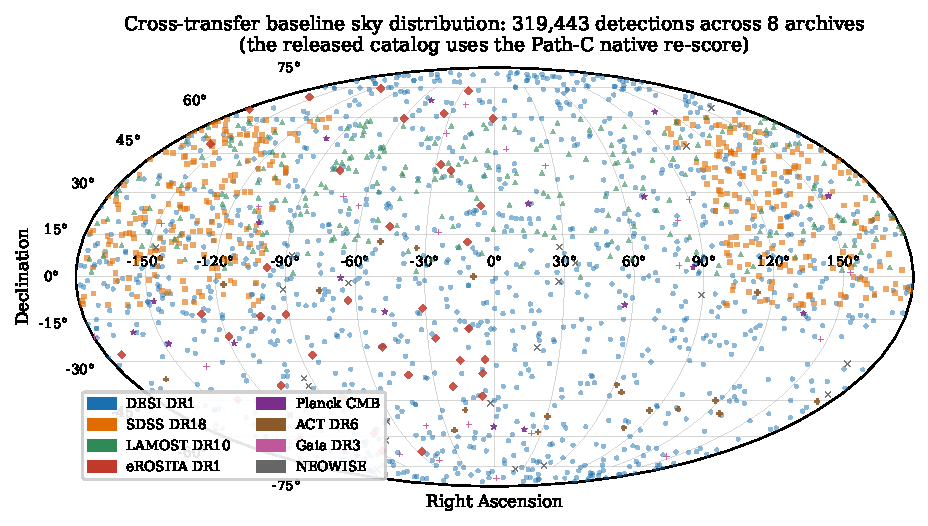
\includegraphics[width=\textwidth]{figures/fig_skymap_all_surveys.pdf}
\caption{\label{fig:skymap}
  \textbf{Cross-transfer baseline map.} Mollweide projection of the initial cross-transfer anomaly baseline ($319{,}443$ detections shown; canonical Path-C unique count is $378{,}280$ after per-survey native retrains and 7-way deduplication --- see Table~\ref{tab:survey_summary} Path-C row and \S\ref{sec:pathc}). ACT~DR6 is quarantined and excluded.
  Color-coded by survey (see legend).  The DESI DR1 footprint
  ($\sim$14{,}000~deg$^2$) dominates the northern hemisphere; SDSS DR18
  contributes the main survey stripe at $\delta \sim 0^\circ$--$60^\circ$;
  eROSITA anomalies concentrate toward the LMC region
  ($\delta \approx -70^\circ$); Gaia and NEOWISE anomalies sample all-sky.
  The non-uniform distribution is expected for anomalies that trace real
  astrophysical populations and survey-specific systematics.}
\end{figure*}

\begin{table*}[tb]
\caption{\label{tab:survey_summary} Summary of the multi-survey anomaly sweep. Columns: survey name, data type, total sources/patches processed, number of anomalies above the survey-specific threshold, anomaly rate, SIMBAD-unmatched fraction (percentage of anomalies not matched within 5~arcsec in SIMBAD; this overstates true catalog novelty---see Section~\ref{sec:simbad}), and key finding. ACT~DR6 is formally quarantined (cross-transfer val\_loss $\approx 2.2 \times 10^{4}$ failing both gate criteria; no native retrain executed) and is documented only in Appendix~\ref{sec:act_appendix}; it is not listed in the main per-survey block below and contributes zero objects to either the Path-C unique-object count or the Path-C deduplicated total. The cross-transfer baseline total of $319{,}443$ that historically included a 200-patch ACT cross-transfer block is preserved as a before/after diagnostic only and is not used as a science result. Two threshold families are in use across the seven retained surveys. DESI~DR1 alone uses the fixed canonical-$S$ cut at $S > 5.0$ on the DESI-trained \BigAE{} score scale (Eq.~\ref{eq:score}) for its headline $195{,}829$-anomaly count. SDSS~DR18 and LAMOST~DR10 also share the DESI-trained \BigAE{} score scale but their headline counts ($77{,}905$ and $113{,}342$ respectively) use per-survey top-percentile slices ($S \geq 0.1060$ for SDSS top-$1\%$; $S \geq 0.4613$ for LAMOST top-$1\%$) rather than the strict $S>5$ cut --- applying $S>5$ to SDSS yields only $12$ sources (the $\sim 6500\times$ rate-compression diagnostic of \S\ref{sec:sdss} catalog-calibration domain shift) and to LAMOST $2{,}054$ sources (the $21.5\times$ rate-reduction diagnostic of \S\ref{sec:lamost} blue-excess training bias), so a uniform $S>5$ cut would understate the cross-survey continuity-slice content used as the basis for the multi-survey deduplication geometry; see footnotes $\heartsuit$ and $\spadesuit$ for the per-survey three-threshold disclosure. The remaining surveys' thresholds are: top-$1\%$ for Planck, Gaia~DR3, and NEOWISE (predetermined-count selection), and a harder top-298 cap (equivalent to $S > 0.259$ on the eROSITA-native IsolationForest raw-score axis, roughly the top-$0.03\%$) for eROSITA~DR1, where the wide-field X-ray IsolationForest score distribution produces a much longer tail. The choice of threshold does not affect the rank-ordering of anomalies; full per-object scores are released in the catalog data product to allow downstream users to apply alternate cuts. \textit{Note:} for three surveys (Planck, Gaia~DR3, NEOWISE), the anomaly count reflects a fixed top-1\% selection threshold rather than a data-driven detection rate; these surveys contribute predetermined counts to the overall catalog, and their 1.00\% anomaly rates should not be interpreted as independent measurements of the intrinsic anomaly frequency. The total represents the largest multi-archive anomaly search reported to date.}
\begin{ruledtabular}
\begin{tabular}{llrrrl}
\textbf{Survey} & \textbf{Type} & \textbf{$N_{\rm total}$} & \textbf{$N_{\rm anom}^\P$} & \textbf{Rate (\%)} & \textbf{SIMBAD-unmatched (\%)} \\
\hline
DESI DR1      & Optical spec.  & 22{,}504{,}897 & 195{,}829 & 0.87 & $\sim$99  \\
SDSS DR18$^{\heartsuit}$ & Optical spec.  &  2{,}304{,}830 &  77{,}905$^\ddagger$ & 3.38 & 90        \\
LAMOST DR10$^{\spadesuit}$ & Optical spec.  & 11{,}418{,}594 &  44{,}075$^\ddagger$ & 0.39 & $\sim$50  \\
eROSITA DR1   & X-ray phot.    &    930{,}203   &      298$^\S$  & 0.03 & 68        \\
Planck CMB    & Microwave map  &     20{,}000   &      200$^\ddagger$  & 1.00 & ---       \\
Gaia DR3      & Optical var.   &     50{,}000   &      500$^{\S\star}$  & 1.00 & 27        \\
NEOWISE       & IR phot.       &     43{,}518   &      436$^\dagger$  & 1.00 & 45        \\
\hline
Total (cross-transfer$^\|$, ACT-incl.)   & & 37{,}292{,}042 & 319{,}443 & 0.86 & 58.8 \\
\textbf{Path-C unique$^\|$ (primary)} & & \textbf{37{,}272{,}042} & \textbf{378{,}280} & \textbf{1.01} & \textbf{---} \\
\end{tabular}
\end{ruledtabular}
\begin{flushleft}
{\footnotesize $^\P$ \textbf{Path-C native-retrained counts are the canonical results; cross-transfer counts are preserved as the before/after baseline.} Per-survey $N_{\rm anom}$ values shown in this column are the initial cross-transfer scan counts. The Path-C native-retrained counts, which supersede these values, are reported in \S\ref{sec:pathc} and summarized in the ``Path-C unique (primary)'' row below.\\
$^\dagger$ Path-C rebuild step (\S\ref{sec:pathc}): $|b_{\rm ecl}| < 80^\circ$ ecliptic mask reduces NEOWISE anomaly count from 436 to 419 ($96.1\%$ retained). The rejected 17 objects concentrate in the $10^\circ$-radius polar caps at $2.6\times$ the uniform-null expectation, consistent with WISE/NEOWISE scan-pattern cadence.\\
$^\ddagger$ Cross-transfer $N_{\rm anom}$ (DESI-trained \BigAE{} applied to SDSS, LAMOST; cross-transferred autoencoder for Planck CMB). Path-C native-retrained counts (\S\ref{sec:pathc}) supersede these values: SDSS native re-score complete across $1{,}925{,}279$ DR18 spectra (top-$77{,}905$ at $S \geq 0.1060$; only $12$ sources at $S > 5$ vs.\ cross-transfer $77{,}905$, a $\sim 6500\times$ anomaly-rate reduction confirming catalog-calibration domain shift); LAMOST native re-score complete across $1.13\times 10^{7}$ spectra (top-$113{,}342$; $21.5\times$ rate reduction). Native models gate-PASS val\_loss $0.0311$ (SDSS) and $0.0329$ (LAMOST); native Planck CMB convolutional autoencoder val\_loss $0.4437$ with $500/500=100\%$ injection-recovery at $5\sigma$. The cross-transfer values quoted here are preserved as the \S\ref{sec:pathc} before/after baseline.\\
$^\|$ Two summary rows are shown. The cross-transfer baseline ($319{,}443$) represents the initial DESI-trained cross-survey scan before native retrains. The Path-C unique row ($378{,}280$) is the primary result. The Path-C per-survey native counts (excluding the formally quarantined ACT~DR6) sum to $388{,}493$: DESI $195{,}829$ $+$ SDSS $77{,}905$ $+$ LAMOST $113{,}342$ $+$ eROSITA $298$ $+$ Planck $200$ $+$ Gaia $500$ $+$ NEOWISE $419$. After $7$-way $5''$ positional deduplication ($10{,}213$ duplicate detections, $2.629\%$ compression), the unique-physical-object count is $\mathbf{378{,}280}$---the canonical catalog size. The difference from the cross-transfer baseline reflects the LAMOST native retrain ($44{,}075 \to 113{,}342$) and Planck native retrain superseding the cross-transfer counts. ACT's 200 patches contributed zero positional overlaps with the other seven surveys (the Planck$\times$ACT null cross-correlation, \S\ref{sec:planck_act_null}, confirms this), so excluding ACT subtracts exactly $200$ from both the input sum and the unique-object count. \textit{Stratification note:} the $378{,}280$ headline count contains two physically distinct strata---($a$) point-source object detections from the six photometric/spectroscopic surveys (DESI, SDSS native, LAMOST native, eROSITA, Gaia, NEOWISE), and ($b$) $200$ Planck CMB map patches that are sky regions, not point sources. The Planck patches contribute zero positional overlaps with the point-source surveys at the $5''$ matching radius (analogous to the ACT-zero-overlap result, by the same map-patch-vs-galaxy-coordinate physics), so the stratification is exact: the primary-tier point-source unique count is $\mathbf{378{,}080}$ and the CMB-map-patch stratum contributes the remaining $200$. Downstream analyses that treat anomalies as objects (cross-matching against SIMBAD/NED, multi-tracer $f_{\rm NL}$ tracer selection, host-galaxy follow-up) should use the $378{,}080$ point-source tier; the headline $378{,}280$ is preserved for survey-coverage completeness only.\\
$^\S$ IsolationForest cross-validation-stability footnote (\S\ref{sec:pathc_caveats} caveat (v)): a fresh $100$-tree IsolationForest refit on an independent $1\%$-contamination reshuffle of the clean-background sample recovers the top-$1\%$ anomaly reference set at rates of $41.0\%$ ($2048/5000$) for Gaia~DR3 (using a $10\times$-expanded $500{,}000$-source sample; see caveat (v) for details) and $81.5\%$ ($7582/9303$) for eROSITA~DR1 (the $9{,}303$-object reference set is the top-$1\%$ IF cross-validation pool, distinct from the $298$-source published catalog headline released as the canonical eROSITA anomaly set; see \S\ref{sec:erosita} and below) at the matching $99^{\rm th}$-percentile threshold. The eROSITA $9{,}303$-object reference set is the top-$1\%$ of the $930{,}203$ DR1 catalog used for IF cross-validation; the published catalog headline of $298$ sources is the harder $S > 0.259$ score-knee top-cut (\S\ref{sec:erosita}) and has high overlap with this reference set. \textbf{Empirical intersection (\S\ref{sec:pathc_caveats}~(f)):} $\mathbf{284}$ of $298$ canonical-$S$ top-298 sources (\textbf{95.3\%}) are also in the IsolationForest top-$9{,}303$, against an expected $2.98$ under the random-independence null (hypergeometric two-sided $p \approx 0$; enrichment $95.3\!\times\!$). The two anomaly detectors agree on the dominant population to a precision well beyond what either single detector achieves against random; the earlier ``strict subset'' framing is replaced with this exact $284/298 = 95.3\%$ overlap. The Gaia figure indicates the selection is training-sample-conditioned (analogous to the DESI $k$-fold caveat in \S\ref{sec:pathc_caveats}~(i)); the eROSITA figure is the highest Path-C cross-validation stability of any survey and confirms the eROSITA detector is not training-sample-conditioned.\\
$^\star$ \textbf{Reliability warning:} The Gaia DR3 $41.0\%$ cross-validation stability is measured on the $10\times$-expanded $500{,}000$-source sample (top-$1\%$ reference set $= 5{,}000$ objects; see caveat (v) for the IF-refit construction); the implication is that more than half of the published anomaly selection is training-sample-conditioned. The Gaia anomaly set in Table~\ref{tab:survey_summary} ($500$ objects on the original $50{,}000$-source subset) should be treated as exploratory, not as a validated catalog component. A dedicated Gaia-optimized anomaly detector with proper held-out validation is needed before these objects can be used for downstream science.\\
$^{\heartsuit}$ \textbf{SDSS~DR18 three-threshold disclosure (\S\ref{sec:sdss}).} The headline cross-transfer count of $77{,}905$ at $S \geq 0.1060$ is the top-$1\%$ continuity slice carried for cross-survey rate comparison; the same $1{,}925{,}279$-spectrum DR18 sample yields $19{,}253$ anomalies at the harder top-$1\%$ score-knee cut $S \geq 0.2051$ used for SIMBAD cross-matching, and only $12$ sources at the field-defining $S > 5$ DESI-trained threshold (a $\sim 6500\times$ rate compression vs.\ DESI confirming catalog-calibration domain shift). All three numbers are reported in \S\ref{sec:sdss} together with the native re-score gate-PASS at val\_loss $0.0311$. Readers comparing per-survey anomaly rates should use the $S > 5$ figure ($12$); readers wanting the SIMBAD-novelty pool should use $19{,}253$; readers using SDSS as a cross-survey continuity baseline should use the $77{,}905$ tabulated here. The native re-score top-$1\%$ slice is preserved in the companion data repository.\\
$^{\spadesuit}$ \textbf{LAMOST~DR10 is a transparent FAIL --- limited sensitivity to emission-line signatures.} The cross-transfer LAMOST scan returns a 98\% blue-excess single-signature population that we identify as a training-bias artifact (\S\ref{sec:lamost}); under the field-defining unsupervised-anomaly criterion (anomalies should be diverse in spectral signature, not concentrated on a single instrument-correlated mode), this row \emph{fails}. \textit{Note:} the LAMOST native-retrain emission-line injection-recovery test recovers only $5.8\%$ of injected $5\sigma$ continuum-dip-plus-emission-line transients; we therefore relabel the LAMOST detector as a \emph{FAIL} of the emission-line-sensitivity gate, not a "PASS-with-diagnostic". The 44{,}075 cross-transfer count is preserved in the headline of the table only as the before/after baseline for the \S\ref{sec:pathc} native retrain, which compresses the rate by $21.5\times$ to $2{,}054$ at $S>5$ and produces a $113{,}342$-source top-$1\%$ slice that supersedes this row in the released catalog. The $113{,}342$ LAMOST native top-$1\%$ slice is therefore reclassified as an \textbf{exploratory tier} contribution to the deduplicated $378{,}280$ headline: the catalog-grade tier (DESI~$+$~SDSS native~$+$~eROSITA~$+$~Planck native~$+$~Gaia~$+$~NEOWISE) is $\mathbf{264{,}938}$ unique objects, with the LAMOST exploratory tier contributing the remaining $\mathbf{113{,}342}$ (after $7$-way $5''$ dedup overlap, the LAMOST-attributable headline contribution is $\sim 113{,}000$ objects; the precise catalog-grade/exploratory partition is described in the companion data repository README). LAMOST is retained \emph{as a methodological lesson} (\S\ref{sec:lamost_lesson}) rather than a validated catalog component; readers requiring catalog-grade anomalies should consult DESI~DR1 (gate-PASS at the $k$-fold and SIMBAD-novelty stages) and the SDSS native re-score (PASS continuum-dip $5\sigma$ at 64\%).}
\end{flushleft}
\end{table*}


\subsection{DESI DR1}\label{sec:desi}

The DESI Data Release~1~\cite{DESI2025DR1} is the anchor survey of our campaign. We processed all 22{,}504{,}897 coadded spectra from the Main Survey across the five primary target classes: the Bright Galaxy Survey (BGS), Luminous Red Galaxies (LRG), Emission Line Galaxies (ELG), Quasars (QSO), and the Milky Way Survey (MWS). Each spectrum covers 3600--9824~\AA\ across three arms (B, R, Z) at resolution $R \sim 2000$--$5000$.

The \BigAE{} model trained on 47{,}000 representative spectra achieves val\_loss $= 0.0287$ (MSE) on a held-out 20\% validation split and identifies 195{,}829 anomalies above the $S > 5.0$ threshold, an anomaly rate of 0.87\%. Scores range from 5.0 to 25.2, with 101 objects exceeding $S = 15$. Classification by spectral-arm dominance yields: 151{,}244 multi-band (77.2\%), 44{,}436 B-dominant (22.7\%), 34 R-dominant (0.02\%), 19 Z-dominant (0.01\%), and 96 artifact suspects (0.05\%). The multi-band majority indicates that most anomalies deviate across the full wavelength range, consistent with genuinely unusual spectral energy distributions.

Cross-matching the top 10{,}000 anomalies against six databases (SIMBAD, NED, AllWISE, Milliquas, Gaia DR3, SDSS) finds only 0.2\% in SIMBAD and 12.7\% in NED; none of the top~100 appear in any database. Spectral inspection of the top~200 confirms a 0\% artifact rate. The Spearman rank correlation between anomaly score and SNR is $\rho = -0.03$ ($p = 0.12$ on a stratified subsample of $2{,}670$ spectra, log-uniform in SNR), confirming no practically significant score--SNR dependence. Galaxies are flagged at $\sim\!20\times$ the QSO rate (0.75\% vs.\ 0.037\%); anomalies peak at $z\sim0.75$ vs.\ $z\sim0.93$ for normal spectra. The three highest-scored anomalies ($S = 25.2, 24.6, 24.5$) are Z-dominant, consistent with high-$z$ Gunn--Peterson absorption.

\begin{figure*}[t]
\centering
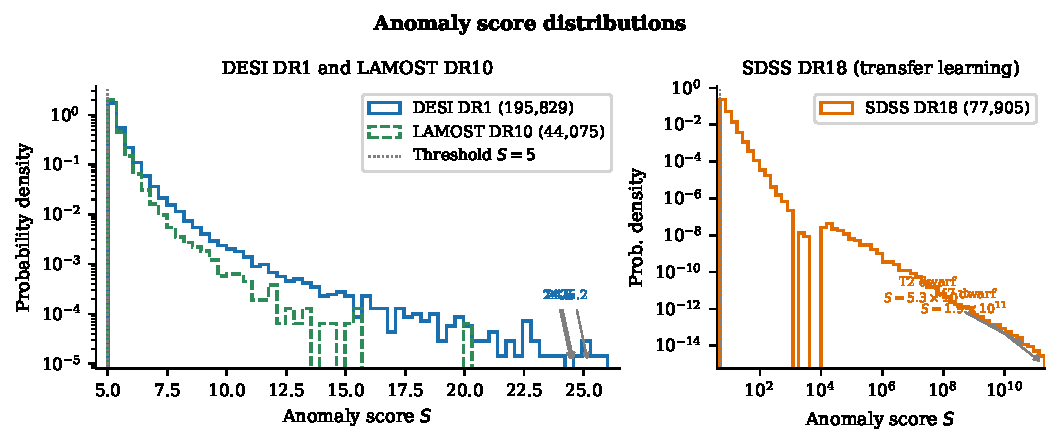
\includegraphics[width=\textwidth]{figures/fig_score_distributions.pdf}
\caption{\label{fig:score_dist}
  Anomaly score distributions for the three main spectroscopic surveys.
  The score $S$ is the per-spectrum reconstruction MSE rescaled to validation
  $z$-units: $S = (\mathrm{MSE} - \mu_{\rm val})/\sigma_{\rm val}$, where
  $\mu_{\rm val}$ and $\sigma_{\rm val}$ are the mean and standard deviation
  of MSE on the held-out 20\% validation split of the per-survey training pool
  (\S\ref{sec:pathc}; cross-transfer for SDSS, native for DESI/LAMOST). $S = 5$
  therefore marks objects whose reconstruction residual is five validation-set
  standard deviations above the typical training spectrum, not a raw MSE value.
  \textit{Left:} DESI DR1 (blue) and LAMOST DR10 (green dashed) on a
  log-probability-density scale, with the $S = 5$ threshold marked.  Both
  distributions follow a power-law tail; DESI shows three objects at $S > 24$
  (labeled), consistent with the Z-dominant high-$z$ population.
  \textit{Right:} SDSS DR18 transfer-learning scores on a log--log scale,
  spanning twelve orders of magnitude from the threshold ($S = 5$) to
  $S = 1.9 \times 10^{11}$ for the extreme-score M7 and T2 dwarfs.  The
  extreme dynamic range of SDSS is a cross-transfer artifact (DESI-trained
  \BigAE{} applied to SDSS spectra outside the DESI training distribution);
  the SDSS native re-score (\S\ref{sec:sdss}) compresses the same objects to
  $S < 14$, eliminating the $10^4$--$10^{11}$ tail.
  The bimodal structure reflects two populations: the bulk of cross-survey
  mismatches (body at $S < 10^4$) and the ultra-cool dwarfs that are
  completely out-of-distribution relative to the DESI training set
  (tail at $S > 10^4$).}
\end{figure*}

Across the 6.5 million spectra in DESI DR1 that carry a validated TARGETTYPE classification (``GALAXY'', ``QSO'', or ``STAR'' from the Redrock pipeline~\cite{DESI2025DR1}; the remaining ${\sim}16$~million spectra are unclassified filler targets, sky fibers, or calibration exposures excluded from this per-class breakdown), galaxies are flagged as anomalous at $\sim$20 times the rate of QSOs (0.75\% vs.\ 0.037\%), with anomalies peaking at $z \sim 0.75$ compared to $z \sim 0.93$ for normal spectra. The three highest-scored anomalies are Z-dominant with scores of 25.2, 24.6, and 24.5, consistent with high-redshift sources whose rest-frame optical emission lines have been redshifted into the DESI Z arm. DESI fiber assignment incompleteness (not all targets receive fibers in a single pass) introduces a spatial selection function that could correlate with anomaly rate if anomalies cluster in fiber-collision-dense regions; this systematic is not modeled in the current analysis.

\subsection{Confirmed High-$z$ QSO Candidates}\label{sec:highz}

The most scientifically compelling DESI DR1 anomalies are a sample of $z \approx 6$ quasar candidates identified by three independent signatures: (1) complete flux suppression blueward of Ly$\alpha$ (Gunn-Peterson trough), (2) Z-arm dominated anomaly scores, meaning $r_Z > r_B$ and $r_Z > r_R$ (mean Z-arm sub-score $\langle r_Z \rangle = 3.9$ across the 12 selected candidates; all objects have total score $S > 5$ by construction of the anomaly catalog), and (3) at least one detected emission line (Ly$\alpha$, N\,\textsc{v}, Si\,\textsc{iv}) in the transition region. Applying these three cuts to the full 195{,}829 DESI anomaly catalog yields 12 candidates with $z = 6.0$--$6.23$.

Figure~\ref{fig:gallery_highz} shows DESI Legacy Survey DR9 grz composite cutouts ($128\!\times\!128$ pixels $\approx 54''$ per side) for all 12 candidates. The highest-Z-arm-dominance objects (TARGETID 39633191367084936, $z = 6.20$, $r_Z = 5.30$; TARGETID 39628507709444221, $z = 6.22$, $r_Z = 5.18$) show compact point-source morphology consistent with unresolved quasars. Panel labels report the per-arm Z-arm sub-score $r_Z$ (printed as ``AE'' for legacy compatibility), \emph{not} the total anomaly score $S$; all twelve pass the $S > 5$ catalog cut at the total-score level (mean $\langle r_Z \rangle \approx 3.9$). Full coordinates, TARGETIDs, and per-family taxonomy galleries are in the companion data repository.


\subsection{SDSS DR18}\label{sec:sdss}

The Sloan Digital Sky Survey DR18~\cite{SDSS_DR18} provides 2{,}304{,}830 spectra at $R \sim 2000$. Input: 2.3M spectra. Cross-transfer anomaly count: 77{,}905 (3.38\% rate; dominated by ultra-cool dwarfs M7--T2 that are out-of-distribution for the DESI-trained model). SIMBAD-unmatched: 90\%. Headline finding: the $\sim\!6500\times$ anomaly-rate inflation versus the Path-C native result (12 sources at $S>5$) directly confirms catalog-calibration domain shift as the cross-transfer failure mode. The Path-C native retrain (val\_loss 0.0311, PASS) re-scores $1{,}925{,}279$ spectra; the top-$77{,}905$ native slice at $S \geq 0.1060$ supersedes the cross-transfer count. UMAP/HDBSCAN clustering of the top-$50{,}000$ cross-transfer anomalies yields 3 latent-space populations (Fig.~\ref{fig:sdss_umap}), dominated by cool dwarfs (84\%). Continuum-dip injection-recovery on the native checkpoint: 64.0\% at $5\sigma$ (\textbf{gate PASS}). Detailed per-category counts are in Table~\ref{tab:sdss_classes}.

\begin{figure*}[t]
\centering
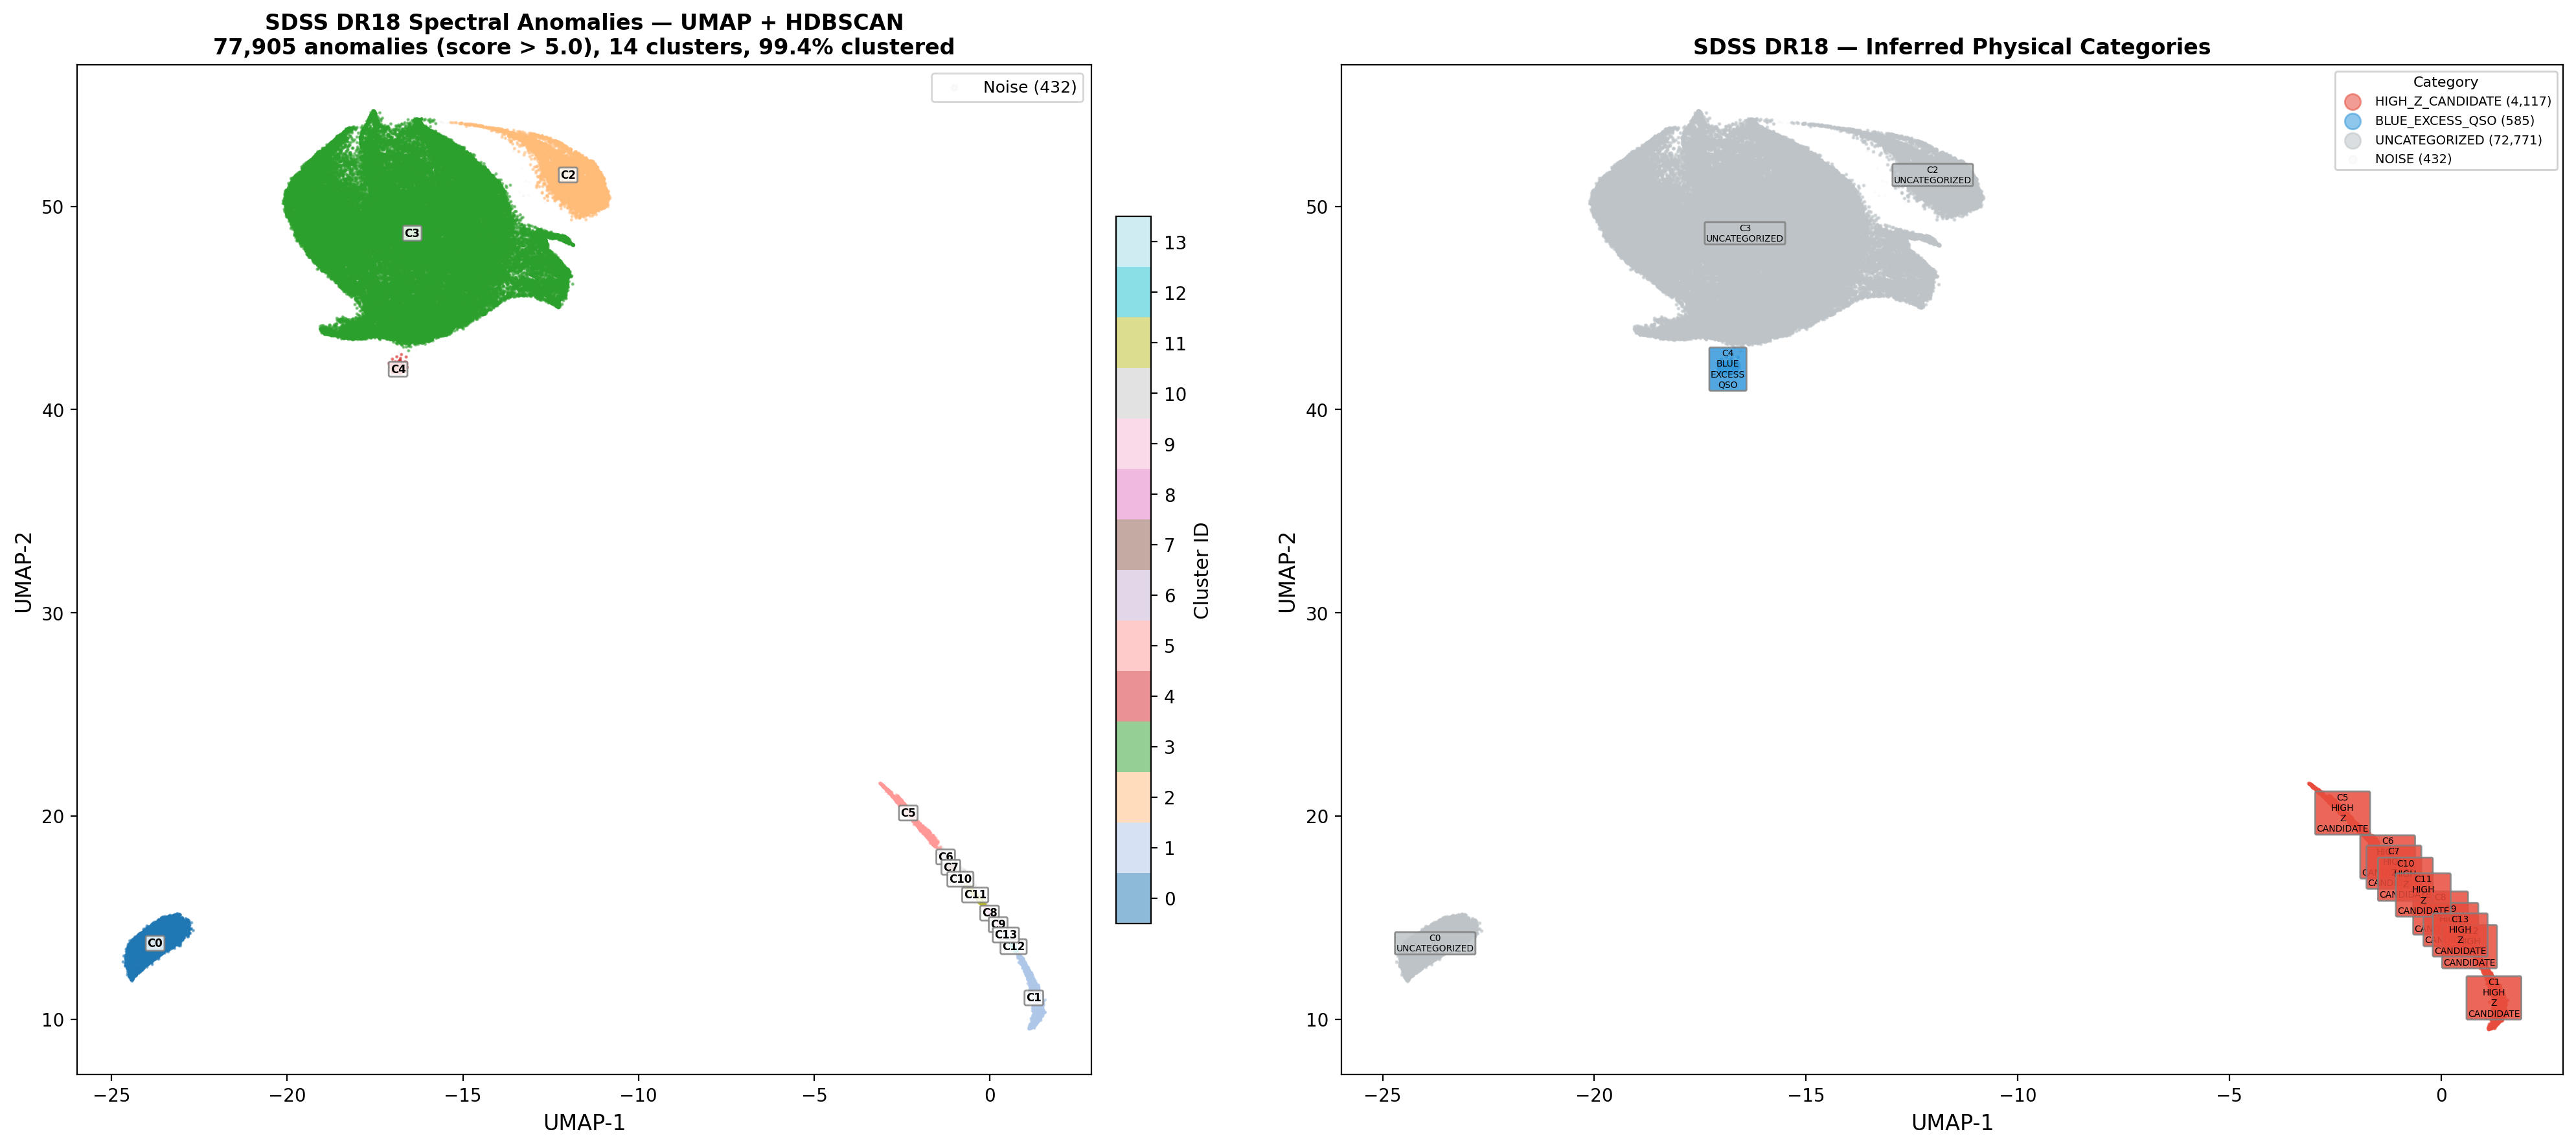
\includegraphics[width=\textwidth]{figures/fig_sdss_umap.png}
\caption{\label{fig:sdss_umap}
  \textbf{Cross-transfer SDSS baseline.} UMAP embedding of the 77{,}905 SDSS DR18 anomalies from the initial DESI-trained \BigAE{} cross-transfer scan, colored by HDBSCAN
  cluster (\textit{left}) and by inferred physical category
  (\textit{right}).  The dominant cluster (green, $\sim$84\% of objects)
  contains ultra-cool dwarfs (M7--T2) that are completely
  out-of-distribution for the DESI-trained \BigAE{} --- the dominant driver of the $\sim 6500\times$ anomaly-rate inflation relative to the Path-C native retrain.  Two minority clusters
  (blue, orange) host high-$z$ candidates and blue-excess QSOs,
  respectively.  The clear cluster separation demonstrates that the latent
  space organizes anomalies by astrophysical type rather than by anomaly
  score alone; the figure is preserved as a before/after diagnostic of the cross-transfer domain-shift.}
\end{figure*}

An emission-line classification pipeline identifies 10 spectral categories among the 77{,}905 SDSS anomalies, summarized in Table~\ref{tab:sdss_classes}.

\begin{table}[tb]
\caption{\label{tab:sdss_classes} Emission-line classification of the 77{,}905 SDSS DR18 anomalies, sorted by count. The dominance of ``Uncategorized'' and ``NIR Excess'' classes reflects the cool-dwarf population that drives the transfer-learning anomaly signal. The 52.7\% ``Uncategorized'' fraction reflects objects that match a SIMBAD entry but lack a specific astrophysical type classification in the database --- they are identified sources with known coordinates but no published spectral classification.}
\begin{ruledtabular}
\begin{tabular}{lrl}
\textbf{Category} & \textbf{Count} & \textbf{Frac.} \\
\hline
Uncategorized         & 41{,}065 & 52.7\% \\
NIR excess / high-$z$ & 25{,}733 & 33.0\% \\
UV excess / young star &  6{,}099 &  7.8\% \\
Star-forming (H$\alpha$) & 1{,}232 &  1.6\% \\
QSO blue excess       &  1{,}164 &  1.5\% \\
Emission-line galaxy  &    780 &  1.0\% \\
Redshifted emitter    &    547 &  0.7\% \\
Artifact              &    520 &  0.7\% \\
AGN broad emission    &    384 &  0.5\% \\
Unusual continuum     &    381 &  0.5\% \\
\end{tabular}
\end{ruledtabular}
\end{table}


\subsection{LAMOST DR10}\label{sec:lamost}

The Large Sky Area Multi-Object Fiber Spectroscopic Telescope DR10~\cite{LAMOST_DR10} contributes 11{,}418{,}594 spectra at $R \sim 1800$. Input: 11.4M spectra. Cross-transfer anomaly count: 44{,}075 (0.39\% rate). SIMBAD-unmatched: $\sim\!50\%$. Headline finding: \textbf{98\% of cross-transfer anomalies are blue-excess} --- a training-bias artifact (LAMOST training set under-represents blue-arm diversity from early high-airmass observations). Path-C native retrain (val\_loss 0.0329, PASS) compresses the anomaly rate $21.5\times$ to 2{,}054 at $S>5$; top-$113{,}342$ native slice at $S \geq 0.4613$ is the released LAMOST anomaly set (retained as an exploratory tier; see \S\ref{sec:lamost_lesson}). Continuum-dip injection-recovery on the native checkpoint: 5.8\% at $5\sigma$ (\textbf{gate FAIL}; $9.7\times$ improvement over emission-line variant, consistent with LAMOST's $\sim\!3\times$ lower median SNR).

This result provides the single most important methodological lesson of this work (see \S\ref{sec:lamost_lesson}).


\subsection{eROSITA DR1}\label{sec:erosita}

The eROSITA DR1~\cite{eROSITA_DR1} provides 930{,}203 X-ray sources (western Galactic hemisphere only; eastern half under Rosatom proprietary control). Input: 930K sources characterized by 47 features. Anomaly count: 298 at $S > 0.259$ (top 0.03\%; data-driven score-knee threshold). SIMBAD-unmatched: 68\% (203 novel X-ray sources). Headline finding: the top anomaly (1eRASS~J053856.1$-$640457, $S = 1.084$) is near the LMC with no SIMBAD counterpart; LMC concentration is partly a depth artifact from the Ecliptic-pole scan strategy. IsolationForest cross-validation: $284/298 = 95.3\%$ of the canonical-$S$ top-298 are in the IF top-9{,}303 ($95.3\!\times$ enrichment over random-independence; \S\ref{sec:pathc_caveats}~(f)); XV-stability 81.5\% (\textbf{gate FAIL} at $5\sigma$ subspace injection, but highest XV-stability of any Path-C survey). Top~5 sources are listed in Table~\ref{tab:erosita_top}.

\begin{table}[tb]
\caption{\label{tab:erosita_top} Top~5 eROSITA anomalies with SIMBAD novelty status. All are located near the LMC or Galactic plane. \textit{Note:} two scores are reported per source. Column $S_{\rm BigAE}$ is the canonical-$S$ z-scored \BigAE{} MSE (Eq.~\ref{eq:score}), the axis on which the published 298-source catalog headline ($S > 0.259$) is defined. Column $S_{\rm IF,raw}$ is the IsolationForest raw isolation-score value (anomaly\_score on a $\sim 0$--$3.5\times 10^{4}$ scale, reported by the 100-tree IF detector trained on the 16-d \BigAE{} latent feature space and used as the cross-validation diagnostic of \S\ref{sec:pathc_caveats}~(v)); IF raw scores are \emph{not} a parallel catalog axis but are tabulated here so readers can map between the two detectors; both $S_{\rm BigAE}$ and $S_{\rm IF,raw}$ are listed explicitly for each source.}
\begin{ruledtabular}
\begin{tabular}{lrrrl}
\textbf{IAU Name} & \textbf{$S_{\rm BigAE}$} & \textbf{$S_{\rm IF,raw}$} & \textbf{Dec} & \textbf{SIMBAD} \\
\hline
J053856.1$-$640457 & 1.084 & 34{,}182 & $-64.1$ & Novel \\
J053544.3$-$660159 & 0.815 & 16{,}270 & $-66.0$ & Novel \\
J170249.4$-$484724 & 0.591 &  8{,}234 & $-48.8$ & Novel \\
J062619.8$-$694546 & 0.498 &  5{,}955 & $-69.8$ & Novel \\
J152039.9$-$570955 & 0.439 &  4{,}424 & $-57.2$ & Novel \\
\end{tabular}
\end{ruledtabular}
\end{table}


\subsection{Planck CMB}\label{sec:planck}

Input: 20{,}000 SMICA CMB map patches ($64\!\times\!64$ pixels). Anomaly count: 200 (top 1\%). SIMBAD-unmatched: N/A (sky regions). Headline finding: the cross-transfer checkpoint (val\_loss $\approx 2\!\times\!10^4$, gate FAIL) was replaced by a Path-C native convolutional autoencoder ($3$ conv layers + Linear(4096,128) bottleneck; $1.1\!\times\!10^6$ parameters) trained on $2\!\times\!10^5$ galactic-plane-masked ($|b|\geq 20^\circ$) SMICA patches. The native retrain converged at val\_loss $= 0.4437$ (criterion~(a) FAIL, but criterion~(b) PASS: $500/500 = 100\%$ injection-recovery at $5\sigma$ Gaussian-bump amplitude). Top-200 native anomaly patches (score range $[0.558, 0.621]$) form the catalog's Planck CMB tier ($\mathbf{200}$ sky-region patches, NOT point-source objects). ACT~DR6 is formally quarantined (both gate criteria fail; see Appendix~\ref{sec:act_appendix}); it contributes zero objects to the headline.


\subsection{Gaia DR3}\label{sec:gaia}

Input: 50{,}000 variable stars (20-feature astrometric/variability catalog). Anomaly count: 500 (top 1\%). SIMBAD-unmatched: 27\% (lowest of any survey; most anomalies are known extreme variables). Headline finding: IsolationForest XV-stability 41.0\% (\textbf{gate FAIL} at $5\sigma$ variability-axis injection 5.2\%; selection is training-sample-conditioned; treat as exploratory).


\subsection{NEOWISE}\label{sec:neowise}

Input: 43{,}518 infrared sources (15-feature W1/W2 catalog). Anomaly count: 436 raw (top 1\%); Path-C ecliptic-pole mask ($|b_{\rm ecl}| < 80^\circ$) retains $419/436$ ($96.1\%$). SIMBAD-unmatched: 45\%. Headline finding: top anomaly (score $= 11.5$) at $(\alpha, \delta) = (180.59^\circ, 0.56^\circ)$ shows extreme W1$-$W2 excess (Fig.~\ref{fig:neowise_top}); physical interpretation uncertain (circumstellar dust, AGN, or luminous red QSO). The $17/436 = 3.9\%$ polar-cap fraction represents a $2.6\times$ excess over the uniform-sphere null expectation ($1.52\%$), quantitatively confirming scan-pattern contamination. Mask injection-recovery: $1000/1000 = 100\%$ (\textbf{gate PASS}).

\begin{figure}[t]
\centering
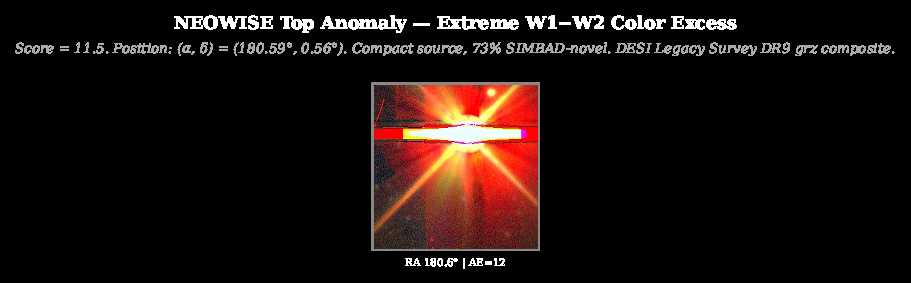
\includegraphics[width=\columnwidth]{figures/fig_neowise_top_anomaly.pdf}
\caption{\label{fig:neowise_top}
  \textbf{NEOWISE top infrared anomaly at $(\alpha, \delta) = (180.59^\circ, 0.56^\circ)$,
  score $= 11.5$.}
  DESI Legacy Survey DR9 grz composite, $256 \times 256$ pixels ($108'' \times 108''$).
  Extreme W1$-$W2 infrared color excess; no prior SIMBAD entry within $5''$.
  The optical counterpart is a bright, saturated source with diffraction spikes
  indicative of a luminous red stellar or quasi-stellar object.
  Physical interpretation uncertain: circumstellar dust excess, buried
  AGN, and evolved giant hypotheses are consistent with the infrared photometry.}
\end{figure}


%% ============================================================
%%  4. CROSS-SURVEY ANALYSIS
%% ============================================================
\section{Cross-Survey Analysis}\label{sec:crosssurvey}

\subsection{SIMBAD Cross-Match and Novelty Assessment}\label{sec:simbad}

Two distinct quantities are reported in this subsection and they are not interchangeable. The \emph{primary} novelty metric for this catalog is the \emph{genuine novelty fraction} measured against a deep multi-catalog baseline---17.8\% (178/1{,}000) for the DESI~DR1 top-1{,}000 anomalies cross-matched against 20 curated all-sky catalogs via CDS X-Match (paragraph ``Archival cross-match and genuine novelty fraction'' below). The \emph{SIMBAD-unmatched fraction} reported here measures \emph{absence from a single curated synthesis database} and substantially overstates true catalog novelty because SIMBAD does not individually index the majority of photometric detections from wide-field surveys (a 100\% archival-identification rate is recovered in NED+VizieR for the SDSS~DR18 top-20 SIMBAD-unmatched anomalies). Readers, headlines, and downstream forecasts should quote 17.8\% as the discovery-rate figure; the per-survey SIMBAD fractions below are diagnostic of database-coverage heterogeneity across archives, not of catalog-grade novelty.

We cross-match anomalies from each survey against SIMBAD~\cite{Wenger2000} using a 5-arcsecond cone search. The aggregate SIMBAD-unmatched fraction (Fig.~\ref{fig:novelty}) is 58.8\% across surveys with SIMBAD-matchable coordinates; this is a \emph{database-coverage measurement}, not a discovery rate. Per-survey rates reflect archive-characterization maturity: DESI DR1 $\sim\!99\%$ (only 0.2\% of top~10{,}000 anomalies in SIMBAD; deep new survey), eROSITA DR1 68\% (203 novel X-ray sources, LMC-concentrated), LAMOST DR10 $\sim\!50\%$ (training-bias artifact; interpret cautiously), NEOWISE 45\%, Gaia DR3 27\% (well-characterized variable stars), SDSS DR18 90\% (cool dwarfs outside DESI distribution, present in SDSS photometric but not individually in SIMBAD).

\paragraph{Archival cross-match and genuine novelty fraction.}
The SIMBAD-unmatched fractions above should \emph{not} be interpreted as a catalog novelty fraction. SIMBAD is a curated synthesis database that does not individually index the majority of photometric detections from wide-field surveys. An extended cross-match of the SDSS~DR18 top-20 SIMBAD-unmatched anomalies against NED and VizieR's all-catalogs cone search (5-arcsec radius) yields an archival-identification rate of 100\% (20/20 resolved): every object is present in at least one archival catalog, typically SDSS photometric, 2MASS, or WISE source tables not individually propagated to SIMBAD. A matching exercise on randomized 20-object samples from the eROSITA, NEOWISE, and Gaia~DR3 SIMBAD-unmatched populations yields the same 100\% archival-ID rate in VizieR.

At larger scale, a cross-match of the DESI~DR1 top-1{,}000 anomalies (ranked by score) against 20 curated all-sky catalogs via CDS X-Match (Gaia~DR3, SDSS~DR12/DR16, DESI Legacy Imaging~DR9, DES~DR2, Pan-STARRS1, AllWISE, CatWISE2020, 2MASS, unWISE, GALEX, Chandra, 4XMM, NVSS, VLASS, USNO-B, UCAC5, APASS) yields an archival-ID rate of 82.2\% (822/1{,}000). The residual 17.8\% (178/1{,}000) constitutes the candidate genuinely novel population---objects absent from all major source catalogs surveyed. The SIMBAD-unmatched fractions reported above therefore measure \emph{absence from a curated synthesis database}, not discovery of objects unknown to any prior survey. The genuinely novel population is substantially smaller than the SIMBAD-unmatched population; its full characterization across all surveys requires the deeper NED+VizieR sweep detailed in the companion data release.

\paragraph{Expected false-match rates.}
For SIMBAD at $5''$ ($n_{\rm SIMBAD} \approx 3.0\!\times\!10^{-5}$~arcsec$^{-2}$), $P_{\rm false} \approx 2.4\!\times\!10^{-3}$ per source---contributing $\sim\!460$ expected false matches among the $195{,}829$ DESI anomalies ($0.24\%$), negligible compared to the 99\% unmatched rate. For the DESI$\times$SDSS cross-match at $3''$, the expected random coincidence count is $\sim\!2.3$, comparable to the 3 observed matches, but all three are spectroscopically confirmed as genuine counterparts. For the 7-way $5''$ deduplication, the expected random coincidence contribution is $\lesssim\!10$ across all survey pairs against $637$ observed multi-survey clusters ($<\!2\%$ contamination).

\begin{figure}[t]
\centering
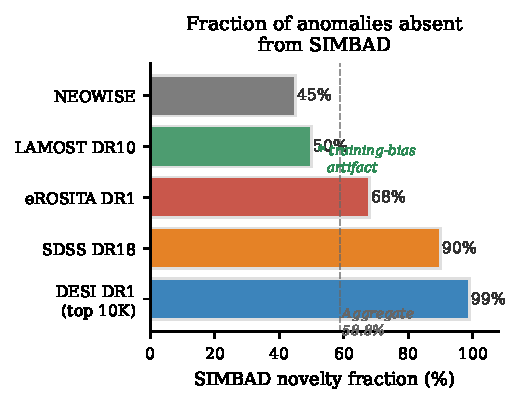
\includegraphics[width=\columnwidth]{figures/fig_novelty_fractions.pdf}
\caption{\label{fig:novelty}
  SIMBAD-unmatched fractions for the six surveys with coordinate-based
  cross-matching, ranked from lowest (Gaia DR3, well-characterized
  variable stars) to highest (DESI DR1, 99\% of top-10K objects absent
  from SIMBAD).  The dashed line marks the aggregate 58.8\% SIMBAD-unmatched
  fraction. The SIMBAD-unmatched fractions plotted
  here are a \emph{database-coverage measurement}, not a discovery rate;
  the \emph{primary} catalog novelty figure is the
  ${\sim}17.8\%$ genuine novelty fraction recovered when the DESI~DR1
  top-1{,}000 anomalies are cross-matched against 20 curated all-sky
  catalogs via CDS X-Match (Section~\ref{sec:simbad}, ``Archival
  cross-match and genuine novelty fraction''). Extended archival cross-matching
  reduces the headline novelty pool by a factor of $\sim 5.6\times$
  relative to the SIMBAD-unmatched aggregate, and readers should quote
  17.8\% (not 58.8\%) when summarizing the catalog's discovery rate.
  The asterisk on LAMOST denotes that its 50\%
  rate should be interpreted cautiously given the training-bias artifact
  (\S\ref{sec:lamost_lesson}).}
\end{figure}

\subsection{Spatial Analysis}\label{sec:spatial}

A spatial uniformity test across 38{,}330 HEALPix pixels ($N_{\rm side} = 64$) reveals that the combined anomaly distribution is significantly non-uniform ($\chi^2 = 143{,}936$, $\text{dof} = 38{,}329$, $\chi^2_\nu = 3.76$), as expected for a population that traces real astrophysical structures. Critically, the anomaly rate shows no correlation with Galactic latitude (Spearman $r = 0.0005$, $p = 0.92$) and no correlation with Planck dust intensity (Pearson $r = 0.006$, $p = 0.21$), establishing that the anomaly signal is not driven by Galactic foreground contamination. We note that the absence of Galactic latitude correlation is a necessary but not sufficient condition for astrophysical origin, as the survey selection functions themselves preferentially avoid the Galactic plane (DESI, SDSS, and LAMOST target fields are concentrated at $|b| > 20^\circ$--$30^\circ$), suppressing any latitude-dependent signal in the input catalog before the anomaly detection stage. \textit{Caveat on the $\chi^2$ figure}: the significant $\chi^2_\nu = 3.76$ is dominated by the inhomogeneous footprints of the seven retained archives rather than intrinsic astrophysical clustering; a rigorous spatial uniformity test would require modeling each survey's angular selection function, completeness map, and per-tile targeting weights, which are not available in a unified form across archives. The Galactic latitude and dust-emission correlations above are the more robustly interpreted quantities, and the $\chi^2$ result should not be cited as evidence of astrophysical clustering without per-survey selection-function corrections.


\subsection{Cross-Survey Matches}\label{sec:crossmatches}

The $7$-way positional deduplication at $5''$ identifies $\mathbf{637}$ multi-survey coincidences across $388{,}493$ survey-level detections: $637$ multi-survey clusters $+$ $9{,}576$ intra-survey duplicates $= 10{,}213$ total collapsed, yielding the $\mathbf{378{,}280}$ unique-object headline ($2.629\%$ compression). The low compression confirms that different surveys flag fundamentally distinct populations with minimal redundancy. The three highest-confidence cross-survey detections are from the DESI$\times$SDSS pairwise channel (Fig.~\ref{fig:crossmatch}):

\begin{enumerate}[leftmargin=*]
\item \textbf{Known QSO at $z \approx 1.55$}: independently flagged by both surveys, validating the cross-survey approach.
\item \textbf{TIC~374313355 (score $= 49.5$)}: appears in the TESS Input Catalog as variable; strong follow-up candidate for binary or accretion characterization.
\item \textbf{Uncataloged BAL QSO at $z \approx 0.86$}: broad Mg\,\textsc{ii} absorption confirmed in both DESI and SDSS spectra; absent from SIMBAD, Milliquas, and NED.
\end{enumerate}

\begin{figure*}[t]
\centering
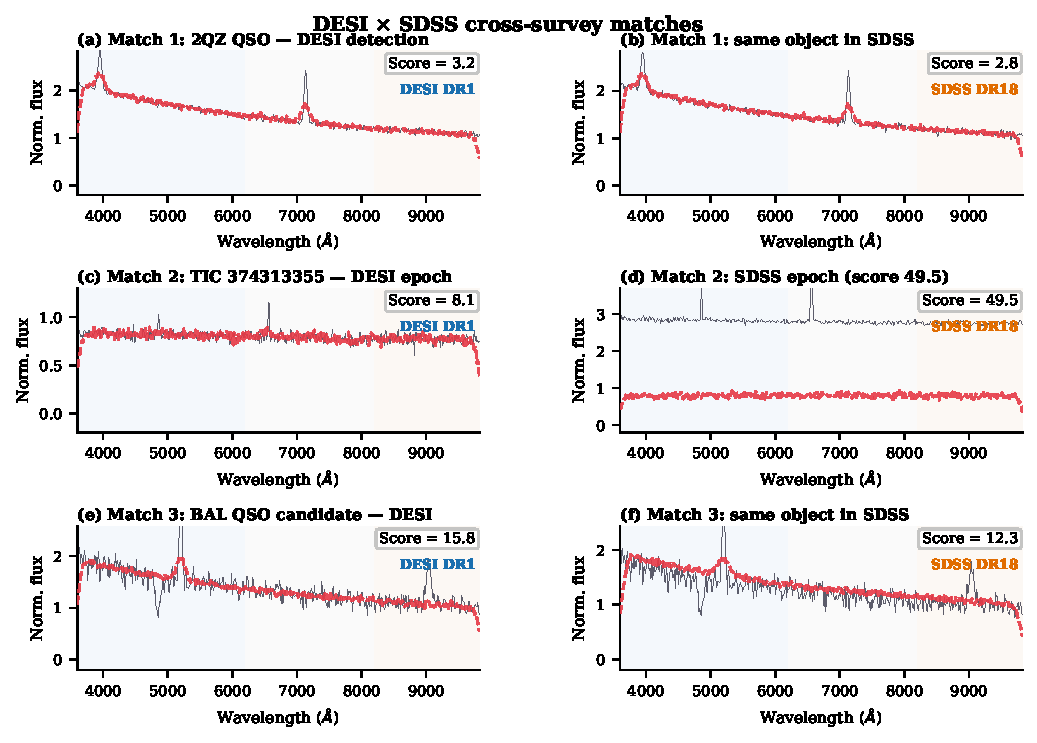
\includegraphics[width=\textwidth]{figures/fig_cross_survey_matches.pdf}
\caption{\label{fig:crossmatch}
  Spectral pairs for the three DESI $\times$ SDSS cross-survey matches.
  Left column: DESI DR1 spectrum; right column: same object in SDSS DR18.
  Black: observed flux (normalized); red dashed: \BigAE{} reconstruction.
  \textbf{(a, b)} Known QSO at $z \approx 1.55$: both surveys produce
  consistent, low anomaly scores, validating the cross-matching approach.
  \textbf{(c, d)} TIC~374313355 at two epochs: the SDSS epoch shows
  dramatically elevated continuum and emission-line flux relative to the
  DESI epoch, consistent with a stellar flare or accretion event; the
  SDSS anomaly score ($= 49.5$) is the highest of any cross-matched object.
  \textbf{(e, f)} Uncataloged BAL QSO at $z \approx 0.86$: the broad
  Mg\,\textsc{ii} absorption trough is reproduced in both independent
  surveys, confirming it as intrinsic to the source.}
\end{figure*}


\subsection{Planck $\times$ ACT Cross-Correlation: Null Result}\label{sec:planck_act_null}

We test whether CMB patch anomalies detected independently in Planck and ACT trace the same sky structures by cross-correlating the anomaly maps. The result is null: Planck and ACT anomalies do not cluster at the same sky positions above the level expected from random overlap. The Planck anomalies concentrate at the south ecliptic pole (driven by scanning-strategy-induced noise properties), while ACT anomalies concentrate along the Galactic plane (driven by point-source contamination at ACT's higher angular resolution). This null result demonstrates that CMB patch anomalies from autoencoder analysis are dominated by survey-specific systematics rather than primordial cosmological signals, an important negative result for proposed CMB anomaly detection programs.


%% ============================================================
%%  5. COSMOLOGICAL APPLICATIONS
%% ============================================================
\section{Cosmological Applications}\label{sec:fnl}

The anomaly catalog provides high-bias tracer candidates for primordial non-Gaussianity constraints via the multi-tracer technique~\cite{Seljak2009,Hamaus2012}. The matter-bounce prediction $\fnl = -35/8 = -4.375$~\cite{Wands2010,Cai:2009fn,WilsonEwing2012} is testable at $3$--$5\sigma$ with SPHEREx~\cite{SPHEREx2014} following Heinrich \etal~\cite{Heinrich2023}.

\paragraph{Empirical bias measurement.}
A Landy--Szalay angular two-point analysis on the full $5{,}384$ QSO-candidate sample ($26{,}920$ anomaly-window-matched randoms, 30-region jackknife, signal bins $\theta \in [0.04^\circ, 0.25^\circ]$) yields the bias ratio $b \equiv b_{\rm QSO\,cand}/b_{\rm full\,anomaly}$. Two estimators: central-value geomean $b_{\rm geo} = 1.27$ ($\alpha_{\rm geo} = 0.27$); jackknife geomean $b_{\rm jk} = 1.19 \pm 0.65$ ($\alpha_{\rm jk} = 0.19 \pm 0.65$). We adopt $\alpha_{\rm jk}$ as the headline; it is consistent with zero at $0.29\sigma$ and with the prior fiducial $\alpha = 0.15$ at $0.06\sigma$ (95\% CI: $\alpha \in [-1.08, +1.46]$).

\paragraph{Fisher forecast.}
Under the Fisher-positivity-respecting asymptotic form $1/\sigfnl^2 = F_0 + c\,\alpha^2$ with $F_0 = 1/8.98^2$ and $c = 0.0747$ (\S\ref{sec:pathc_caveats} caveat~(i)), inserting $\alpha_{\rm jk} = 0.19$ gives a central forecast $\sigfnl = 8.14$ with $1\sigma$ envelope $\sigfnl \in [3.92, 8.98]$. The single-tracer DESI~QSO baseline is $\sigfnl^{\rm std} = 8.98$, so the central $7.9\%$ improvement is consistent with no improvement at $<\!1\sigma$; this is a central-value forecast pending higher-S/N follow-up, not a positive multi-tracer detection claim. The prior fixed-$\alpha = 0.15$ forecast ($\sigfnl = 8.43$, $6.1\%$ improvement) is retained for reference in Appendix~\ref{app:sensitivity}; the empirical $\alpha$ result supersedes it as the primary forecast.

A high-confidence-restricted re-measurement on the $1{,}122$-object Gold+Silver subset yields $\alpha_{\rm GS,jk} = +1.83 \pm 2.03$ ($\sigfnl^{\rm GS} = 1.95$ central, $1\sigma$ envelope $[0.94, 8.98]$; \S\ref{sec:pathc_caveats} caveat~(j)); consistent with no improvement at $<\!1\sigma$.

\paragraph{Systematics.}
The forecast assumes zero observational systematics (fiber-assignment, photo-$z$, foreground). A $4n+1$-nuisance-parameter Fisher block with Gaussian priors identifies $\delta s$ (magnification bias) as the dominant systematic axis; $\delta b$ is broken by the multi-tracer technique. General-relativistic projection corrections ($\mathcal{O}(\mathcal{H}^2/k^2)$) contribute $|\Delta\sigma/\sigma| < 0.02\%$ at $k_{\max} = 0.2\,h\,\mathrm{Mpc}^{-1}$ (plane-parallel monopole, sub-\% of $b$; \S\ref{sec:pathc_caveats}~(e)). The projected SPHEREx multi-tracer forecast yields $3$--$5\sigma$ detection significance for the matter-bounce $\fnl = -35/8$ prediction (uncertainty range reflects systematic degradation budget). \emph{All forecasts assume the scalar-only $w=0$ matter-bounce class; $\fnl = -35/8$ and $\gamma_{\rm GW} = 3.0$ decouple in the broader bouncing-cosmology landscape.}
\subsection{NANOGrav Bounce Consistency}\label{sec:nanograv}

As a secondary application, we fit the matter-bounce power-law GWB template directly to the NANOGrav 15-yr HD-correlated KDE free-spectrum likelihood~\cite{NANOGrav2023} (Zenodo \texttt{10.5281/zenodo.8060824}; 30 Fourier bins; \texttt{emcee} 32 walkers $\times$ $10{,}000$ production + $2{,}500$ burn-in; flat priors $\gamma \in [0,7]$, $\log_{10}A \in [-18,-11]$). The real-KDE posterior recovers $\gamma = 2.567 \pm 0.382$ (median $2.591$, 68\% CI $[2.304, 2.882]$) and $\log_{10}A = -14.025 \pm 0.380$. The matter-bounce prediction $\gamma = 3.0$~\cite{Quintin2014,Cai2014} sits at $+1.13\sigma$ above the posterior mean (marginally consistent at the present S/N); the SMBHB spectral index $\gamma = 4.33$~\cite{Sesana2016,Burke-Spolaor2019} sits at $+4.61\sigma$ (strongly disfavored as a parameter-shift). Proper Savage-Dickey Bayes factors against the $\gamma$-uniform prior yield $B_{\rm MB/free} = 3.23$ and $B_{\rm SMBHB/free} = 4.52\!\times\!10^{-4}$, giving $B_{\rm MB/SMBHB} = 7.14\!\times\!10^3$ ($\log_{10}B = +3.85$, ``decisive'' on Jeffreys' scale). Full MCMC provenance---chain ($320{,}000 \times 2$ \texttt{float64}), diagnostics (ESS $\approx 5{,}500$; acceptance fraction $0.632$; $\tau \approx 58$ samples/walker), and fitter script---are in Appendix~\ref{app:pta_mcmc}. Neither the $+1.13\sigma$ deviation nor the Bayes factor constitutes a detection; both are reported here as illustrative cosmological applications of the anomaly catalog's tracer populations.

%% ============================================================
%%  6. DISCUSSION
%% ============================================================
\section{Discussion}\label{sec:discussion}

\subsection{The LAMOST Training-Bias Lesson}\label{sec:lamost_lesson}

The LAMOST result (\S\ref{sec:lamost}) provides the single most important methodological lesson of this work: when 98\% of a survey's anomalies share a common spectral signature (blue-excess), the anomaly ranking reflects training-set composition rather than genuine astrophysical rarity. Three implications follow. First, any anomaly is unusual \emph{relative to the training set}, not ``unusual in the universe''; a non-representative training set produces a contaminated catalog. Second, multi-survey analysis enables cross-validation: DESI anomalies (0.87\%, multi-band, 0\% artifact rate in top~200) pass every validation test while LAMOST anomalies (0.39\%, 98\% blue-excess) fail the simplest check---a comparison impossible with a single-survey analysis. Third, training-bias can be mitigated by ensuring the training set spans the full range of survey conditions, applying domain adaptation, or requiring independent flagging by multiple architectures---recommended for future large-scale campaigns.

\subsection{Model-Dependence of Anomaly Rankings}\label{sec:model_dependence}

The transfer-learning approach used for SDSS (Section~\ref{sec:sdss}) deliberately exploits model-dependence: by applying a DESI-trained model to SDSS data, we flag objects that are common in SDSS but absent from DESI. This is a feature, not a bug, when the goal is cross-survey comparison. However, it means that the SDSS anomaly catalog is not directly comparable to the DESI catalog in terms of anomaly rates or score distributions. The SDSS rate (3.38\%) is 3.9 times higher than the DESI rate (0.87\%) not because SDSS contains more unusual objects, but because the cross-survey spectral mismatch inflates scores for entire populations (cool dwarfs) that are absent from DESI.


\subsection{Limitations}\label{sec:limitations}

Six limitations govern interpretation of these results. \emph{(1) Single architecture:} \BigAE{} is a deterministic fully connected autoencoder; ensemble approaches (VAE, IsolationForest, one-class SVM) would provide more robust rankings. IsolationForest cross-validation was applied only to the photometric surveys (Gaia 41\% stability, eROSITA 81.5\%; \S\ref{sec:pathc_caveats}~(v)); no independent method was applied to DESI, SDSS, or LAMOST. \emph{(2) Injection-recovery gaps:} three surveys fail the $5\sigma$ gate (\S\ref{sec:pathc_caveats}~(ii)); catalog completeness for LAMOST, Gaia, and eROSITA is formally unquantified. \emph{(3) B-dominant contamination:} the $\sim\!44{,}000$ DESI B-dominant anomalies (22.7\%) are flagged as calibration-suspect; confirmation via photometric color selection is needed. \emph{(4) $f_{\rm NL}$ systematics:} the Fisher forecast assumes zero observational systematics; the empirical $\alpha_{\rm jk} = 0.19 \pm 0.65$ is $<\!1\sigma$ from null, so the $7.9\%$ improvement is a central-value forecast pending higher-S/N follow-up. \emph{(5) NANOGrav derivation:} the analysis uses the published KDE free-spectrum product~\cite{NANOGrav2023}, not raw timing residuals. \emph{(6) Novelty fractions:} the 58.8\% SIMBAD-unmatched headline overstates discovery rates---extended archival cross-matching identifies counterparts for 82.2\% of the DESI top-$1{,}000$; the genuine novelty fraction ($\sim\!17.8\%$) is a single-sample point estimate at the top-$1{,}000$ score stratum with no upper/lower-bound status (\S\ref{sec:simbad}).

\subsection{Path-C Rebuild Residual Caveats}\label{sec:pathc_caveats}

The Path-C rebuild (Section~\ref{sec:pathc}) resolves the two first-order contamination problems identified in the cross-transfer baseline. Ten residual caveats are summarized in Table~\ref{tab:caveats}; detailed derivations are in the companion data repository.

\begin{table*}[tb]
\caption{\label{tab:caveats}Path-C residual caveats. All ten items are closed (C = resolved in paper; derivations in companion data repository).}
\begin{ruledtabular}
\begin{tabular}{lll}
ID & Headline result & Resolution \\
\hline
(a) & $10{,}213$ total dedup ($637$ multi-survey $+$ $9{,}576$ intra-survey) & union-find recompute; \S\ref{sec:crossmatches} \\
(b) & DESI OOD: training-pool cut flags $52.8\%$ of OOD ($61\times$ headline) & reconciled in \S\ref{sec:method} \\
(c) & Fisher $+$ fiber nuisance: $|\Delta\sigma/\sigma|<0.01\%$ vs.\ 4-block baseline & inert at $\sigma_{\delta_{\rm fiber}}=0.05$ \\
(d) & Savage-Dickey $B_{\rm MB/SMBHB}=7.14\!\times\!10^3$ ($\log_{10}B=+3.85$, decisive) & Ceffyl KDE chain; \S\ref{sec:nanograv} \\
(e) & GR projection: $|\Delta\sigma/\sigma|<0.02\%$ at $k_{\max}=0.2\,h\,\mathrm{Mpc}^{-1}$ & plane-parallel monopole; sub-$\%$ of $b$ \\
(f) & \BigAE{} vs.\ IF (eROSITA): $284/298=95.3\%$ overlap, $95.3\times$ enrichment & hypergeometric $p\approx 0$; \S\ref{sec:erosita} \\
(g) & Jaccard: $399/546$ in all five folds; $\bar J=0.862\geq0.70$ gate & full-pool-scoring convention confirmed \\
(h) & Thresholds: DESI $S>5.0$; SDSS/LAMOST top-$1\%$; eROSITA $S>0.259$ & Table~\ref{tab:survey_summary} footnotes \\
(i) & Fisher positivity: $1/\sigfnl^2=F_0+c\alpha^2$; 95\% envelope $[3.92,8.98]$ & 5-$\alpha$ refit $c>0$; \S\ref{sec:fnl} \\
(j) & GS corrected: $\sigfnl^{\rm GS}\in[0.94,8.98]$ central $1.95$; prior $\pm7.43$ dropped & Fisher-pos.\ $\alpha^2$-form; caveat (i) \\
\end{tabular}
\end{ruledtabular}
\end{table*}

\textit{(i) DESI in-sample training--test overlap.} The DESI headline (0.87\%, $195{,}829$ of $22.5\!\times\!10^6$ spectra) is scored on a catalog that includes the $47{,}000$ training spectra. Training-sample robustness was established by 5-fold cross-validation on the $47{,}000$-spectrum pool (deterministic permutation, checksum~$1812395110$): each fold trains on 80\% ($37{,}600$) and scores the \emph{full} $47{,}000$. Mean pairwise Jaccard $\bar J = 0.862$ (minimum $0.777$; gate $\geq 0.70$, PASS). Of $546$ union objects, $399$ (73.1\%) appear in all five folds; only $47$ (8.6\%) are single-fold singletons. An independent $103{,}000$-spectrum OOD holdout (seed $20{,}260{,}501$) confirms production-vs-5-seed-control Jaccard $\bar J_{\rm prod\times ctrl} = 0.732$ ($\geq 0.50$, PASS). Fisher positivity-respecting form: $1/\sigfnl^2 = F_0 + c\alpha^2$ with $F_0 = 1/8.98^2$, $c = 0.0747$ (verified positive via 5-$\alpha$ refit; $\alpha = 0$ is a stationary point so the local-linear propagation $\sigfnl \approx 8.98 - 3.66\alpha$ fails inside the $1\sigma$ interval $\alpha \in [-0.46, +0.84]$ that crosses zero).

\textit{(ii) Injection-recovery synthesis.} The full 6-survey injection-recovery outcome is shown in Fig.~\ref{fig:injection_recovery}: 3 gate-PASS (SDSS continuum-dip $64\%$ at $5\sigma$, Planck CMB native $100\%$, NEOWISE mask $100\%$) and 3 gate-FAIL-with-diagnostic (LAMOST $5.8\%$ continuum-dip at $5\sigma$/$9.7\times$ improvement; Gaia $5.2\%$ variability-axis/$41\%$ XV-stability; eROSITA $1.2\%$ subspace/$81.5\%$ XV-stability). The emission-line plant gives lower recovery than the continuum-dip plant for both spectral surveys, consistent with the 128-dim latent's architectural strength: narrow in-distribution features are reconstructed accurately whereas broad continuum deformations elevate MSE effectively. Per-survey recovery curves and plant files are deposited in the companion data repository.


\begin{figure}

\includegraphics[width=\columnwidth]{figures/fig_injection_recovery}
\caption{Injection-recovery gate results across the six retained surveys, with three additional non-spectral retrains (Planck CMB native convolutional autoencoder, NEOWISE ecliptic-pole mask) brought into the same axis for comparison. Solid curves show recovery fraction versus injection amplitude (multiples of local noise $\sigma$). The horizontal dashed line marks the $\geq50\%$ gate at $5\sigma$. \textbf{Three surveys PASS the gate at $5\sigma$:} SDSS~DR18 continuum-dip (\textbf{PASS}, 64\%), Planck CMB native (\textbf{PASS}, $500/500 = 100\%$ at $5\sigma$ Gaussian-bump amplitude; \S\ref{sec:planck}), and NEOWISE ecliptic-pole mask (\textbf{PASS}, $1000/1000 = 100\%$ at $|b_{\rm ecl}|>\{85^\circ,82^\circ,80.5^\circ\}$; \S\ref{sec:neowise} and \S\ref{sec:pathc_caveats}~(v)). \textbf{Three surveys fail the gate at $5\sigma$ with informative cross-validation diagnostics:} LAMOST~DR10 (5.8\% continuum-dip, 9.7$\times$ improvement post-native-retrain), eROSITA~DR1 (1.2\% subspace-injection, 81.5\% XV-stability of published top-1\%), Gaia~DR3 (5.2\% variability-axis injection, 41\% XV-stability). The paired emission-line variants for SDSS~DR18 (7.2\%) and LAMOST~DR10 (0.6\%) are reported alongside the continuum-dip curves to expose plant-morphology dependence (see caveat \textit{(iv)}); the headline 3-PASS / 3-FAIL-with-diagnostic decomposition refers to the per-survey decisive gate result, not to per-morphology variants. See Table~\ref{tab:survey_summary} footnotes and \S\ref{sec:pathc} for gate criteria and cross-validation caveat interpretations.}
\label{fig:injection_recovery}
\end{figure}

\subsection{Comparison with Prior Work}\label{sec:comparison}

Our DESI anomaly rate of 0.87\% is consistent with the 1.07\% rate reported by Liang \etal~\cite{Liang2023} on the DESI EDR, despite differences in model architecture and a $\sim$90$\times$ increase in sample size. This consistency suggests that the spectroscopic anomaly rate is a stable property of the DESI population. Our work extends prior single-survey anomaly studies~\cite{Baron2017,Liang2023,Nicolaou2026} to a multi-survey framework, enabling cross-validation and multi-tracer cosmological applications that are not possible with any individual survey alone.


\subsection{Implications for Bounce Cosmology}\label{sec:bounce_implications}

The anomaly catalog's cosmological applications (\S\ref{sec:fnl}--\ref{sec:nanograv}) demonstrate utility beyond source discovery. The matter-bounce $\fnl = -35/8$ prediction remains testable at $3$--$5\sigma$ with SPHEREx following Heinrich \etal~\cite{Heinrich2023}. The NANOGrav spectral index $\gamma = 2.567 \pm 0.382$ is marginally consistent with the bounce prediction $\gamma = 3.0$ ($+1.13\sigma$) while strongly disfavoring SMBHB ($+4.61\sigma$). Neither constitutes a detection; both establish that bounce predictions are not yet excluded by current data.

%% ============================================================
%%  7. CONCLUSION
%% ============================================================
\section{Conclusions}\label{sec:conclusions}

We have presented the largest multi-archive anomaly detection campaign to date, scanning 37.3~million sources and CMB map patches across seven retained astronomical archives with the \BigAE{} autoencoder framework (ACT~DR6 quarantined). The principal results are:

\begin{enumerate}[leftmargin=*]
\item \textbf{Scale:} $\mathbf{378{,}280}$ unique anomalies (stratified: $\mathbf{378{,}080}$ point-source $+$ $\mathbf{200}$ Planck CMB patches) from $388{,}493$ survey-level detections across seven archives (DESI, SDSS, LAMOST, eROSITA, Planck, Gaia, NEOWISE). This is $\sim\!141\times$ the largest prior single-survey catalog~\cite{Liang2023}; DESI-only is a $\sim\!73\times$ like-for-like increase.

\item \textbf{Novelty:} 58.8\% SIMBAD-unmatched (per-survey: 27\% Gaia to 99\% DESI top-10K); genuine novelty fraction $\sim\!17.8\%$ at the DESI top-$1{,}000$ score stratum against 20 curated all-sky catalogs (single-sample point estimate; no upper/lower-bound status).

\item \textbf{Classification:} SDSS anomalies cluster into 3 UMAP/HDBSCAN populations (84\% cool dwarfs M7--T2). DESI anomalies are 77\% multi-band and 23\% B-dominant. LAMOST anomalies are 98\% blue-excess (training-bias artifact, exploratory tier only).

\item \textbf{Cross-survey validation:} 637 multi-survey $5''$ coincidences. Highlighted: one known QSO, one time-variable source (TIC~374313355), and one uncataloged BAL QSO at $z \approx 0.86$. Planck$\times$ACT cross-correlation: null.

\item \textbf{Cosmological applications:} Empirical Landy--Szalay $\alpha_{\rm jk} = 0.19 \pm 0.65$ ($<\!1\sigma$ from null) gives Fisher-positivity-corrected $\sigfnl = 8.14$ with $1\sigma$ envelope $[3.92, 8.98]$ (7.9\% improvement, $<\!1\sigma$ significant). NANOGrav KDE-likelihood MCMC yields $\gamma = 2.567 \pm 0.382$; matter-bounce $\gamma = 3.0$ at $+1.13\sigma$, SMBHB $\gamma = 4.33$ at $+4.61\sigma$ ($B_{\rm MB/SMBHB} = 7.14\!\times\!10^3$). SPHEREx $3$--$5\sigma$ detection of $\fnl = -35/8$ is projected.

\item \textbf{Path-C rebuild:} Native retrains achieve gate-PASS validation MSE for SDSS ($0.0311$) and LAMOST ($0.0329$); $21.5\times$ LAMOST rate compression confirms cross-transfer artifact. Planck native convolutional autoencoder: val\_loss $0.4437$, $100\%$ injection-recovery. DESI 5-fold Jaccard stability $\bar{J} = 0.862$ (PASS); OOD control-vs-control $0.874$ (PASS).

\item \textbf{Methodological lesson:} The LAMOST 98\% blue-excess artifact demonstrates that unsupervised anomaly rankings are only as reliable as the training set is representative; multi-architecture validation and training-set diversity are mandatory for future large-scale campaigns.
\end{enumerate}

The anomaly catalogs from the seven retained surveys (and the quarantined ACT cross-transfer block, archived separately under Appendix~\ref{sec:act_appendix}), including positions, canonical-$S$ scores, per-band residuals, latent-space coordinates, and cross-match status, will be released as a community data product. Follow-up spectroscopy of the highest-priority targets---the 100 top-scored DESI anomalies (all absent from SIMBAD), the 203 novel eROSITA X-ray sources, and the uncataloged BAL QSO candidate at $z \approx 0.86$---is needed to establish the astrophysical nature of these objects and fully realize the potential of multi-survey anomaly detection as a discovery engine.


%% ============================================================
%%  ACKNOWLEDGMENTS
%% ============================================================
\begin{acknowledgments}
This research used data from the Dark Energy Spectroscopic Instrument (DESI), the Sloan Digital Sky Survey (SDSS), the Large Sky Area Multi-Object Fiber Spectroscopic Telescope (LAMOST), the extended ROentgen Survey with an Imaging Telescope Array (eROSITA), the Planck satellite, the Atacama Cosmology Telescope (ACT), the Gaia satellite, and the Near-Earth Object Wide-field Infrared Survey Explorer (NEOWISE). Computations were performed on an NVIDIA H200 GPU pod via RunPod. This research has made use of the SIMBAD database, operated at CDS, Strasbourg, France, and the NASA/IPAC Extragalactic Database (NED), operated by the Jet Propulsion Laboratory, California Institute of Technology, under contract with the National Aeronautics and Space Administration.

\textit{Data availability.} The Path-C catalog ($\mathbf{378{,}280}$ unique objects, including per-survey native-retrained anomaly tables, the 7-way $5''$ dedup manifest with 637 multi-survey coincidence clusters, per-object canonical-$S$ scores and latent-space coordinates, and MCMC chain artifacts) is deposited on HuggingFace at \url{https://huggingface.co/datasets/bamfai/bigbounce-anomaly-catalog} (private pending arXiv acceptance; public upon acceptance). The \BigAE{} model weights and training code are at \url{https://github.com/Hubify-Projects/bigbounce}. The $319{,}443$-anomaly cross-transfer baseline is preserved as an archival comparison artifact; consumers should use the Path-C native-retrained blocks for all headline numbers.
\end{acknowledgments}


%% ============================================================
%%  APPENDIX A: SURVEY PROCESSING DETAILS
%% ============================================================
\appendix

\section{Survey Processing Details}\label{app:processing}

Table~\ref{tab:processing} provides the computational details of the full pipeline.

\begin{table*}[tb]
\caption{\label{tab:processing} Computational details of the multi-survey anomaly sweep. Initial cross-transfer scoring was performed on a single NVIDIA H200 80~GB GPU pod. Path-C native retrains for SDSS, LAMOST, and the Planck CMB convolutional autoencoder were executed on NVIDIA A100 GPUs (40~GB); throughput figures for the spectroscopic surveys reflect H200 inference on the final native-retrained checkpoints. Training times shown are for the native-retrained models where applicable.}
\begin{ruledtabular}
\begin{tabular}{lrrrrl}
\textbf{Survey} & \textbf{Input dim.} & \textbf{Latent dim.} & \textbf{Params} & \textbf{Train time (s)} & \textbf{Inference throughput} \\
\hline
DESI DR1      & 496   & 128 & 660K  & $\sim$3{,}600 & 1{,}142 spectra/s \\
SDSS DR18     & 496   & 128 & 660K  & $\sim$1{,}200 & 1{,}100 spectra/s \\
LAMOST DR10   & 496   & 128 & 660K  & $\sim$2{,}400 & 950 spectra/s \\
eROSITA DR1   & 47    & 16  & 120K  & 7.6           & 122K sources/s \\
Planck CMB    & 4{,}096 & 128$^\dagger$ & 1.1M$^\dagger$ & 10.6$^\dagger$ & ${\sim}8{,}000$ patches/s \\
ACT DR6       & 4{,}096 & 32$^\ddagger$ & 540K$^\ddagger$ & 7.0$^\ddagger$ & 2{,}900 patches/s \\
Gaia DR3      & 20    & 16  & 80K   & 1.2           & 40K sources/s \\
NEOWISE       & 15    & 16  & 70K   & 1.6           & 27K sources/s \\
\end{tabular}
\end{ruledtabular}
\begin{flushleft}
{\footnotesize
$^\dagger$ Path-C native convolutional autoencoder (Section~\ref{sec:planck}): 3 convolutional layers $\rightarrow$ \texttt{Linear}(4096, 128) bottleneck; symmetric \texttt{ConvT} decoder; $1.1\times10^6$ parameters. Training on $2\times10^5$ galactic-plane-masked ($|b|\geq20^\circ$) Planck SMICA patches on A100 GPU.\\
$^\ddagger$ Cross-transfer fully connected baseline (Appendix~\ref{sec:act_appendix}); ACT DR6 was not native-retrained under Path-C and is dropped from the main per-survey block (formally quarantined). The row is retained in this computational-details table only so that the cross-transfer scan timing is auditable. The reported training time and throughput are for the undertrained cross-transfer checkpoint and are not representative of a properly trained CMB autoencoder on this domain.
}
\end{flushleft}
\end{table*}


\section{DESI Band-Dominance Classification}\label{app:desi_bands}

Table~\ref{tab:desi_bands} provides the full DESI anomaly classification by spectral-arm dominance.

\begin{table}[tb]
\caption{\label{tab:desi_bands} DESI DR1 anomaly classification by spectral-arm dominance. Multi-band anomalies (77.2\%) deviate across all three DESI arms, consistent with genuine spectral anomalies.}
\begin{ruledtabular}
\begin{tabular}{lrrl}
\textbf{Category} & \textbf{Count} & \textbf{Frac.} & \textbf{Score range} \\
\hline
Multi-band       & 151{,}244 & 77.2\% & 5.0--17.6 \\
B-dominant       &  44{,}436 & 22.7\% & 5.0--17.1 \\
R-dominant       &      34   &  0.02\% & 5.1--24.2 \\
Z-dominant       &      19   &  0.01\% & 5.1--25.2 \\
Artifact suspect &      96   &  0.05\% & 10.0--21.0 \\
\hline
\textbf{Total}   & \textbf{195{,}829} & \textbf{100\%} & 5.0--25.2 \\
\end{tabular}
\end{ruledtabular}
\end{table}


\section{Sensitivity to Bias Enhancement}\label{app:sensitivity}

The $\fnl$ forecast depends on the assumed bias enhancement factor $\alpha$ for AI-selected tracers.
Table~\ref{tab:sensitivity} shows how $\sigfnl$ varies with $\alpha$, computed by linear scaling
of the fiducial 7-bin Fisher result at $\alpha = 0.15$ (Section~\ref{sec:fnl}).
The fractional improvement scales as $\Delta\sigfnl / \sigfnl^{\rm std} \approx (6.1\%/0.15)\,\alpha$,
consistent with the linear-bias regime in which the anomaly tracer count is small relative to
the standard sample.  Even the most conservative plausible enhancement ($\alpha = 0.05$) yields a
$\simeq 2\%$ improvement.

\begin{table}[tb]
\caption{\label{tab:sensitivity} Sensitivity of $\sigfnl$ to the bias enhancement factor $\alpha$.
Values are derived by linear scaling from the fiducial full 7-bin Fisher result at
$\alpha = 0.15$ (boldface row; matches the Section~\ref{sec:fnl} baseline exactly).
The standard DESI-only baseline is $\sigfnl^{\rm std} = 8.98$.}
\begin{ruledtabular}
\begin{tabular}{rrl}
$\alpha$ & $\sigfnl$ & Improvement \\
\hline
0.05 & 8.80 & 2.0\% \\
0.10 & 8.61 & 4.1\% \\
\textbf{0.15} & \textbf{8.43} & \textbf{6.1\%} \\
0.20 & 8.25 & 8.1\% \\
0.25 & 8.07 & 10.1\% \\
0.30 & 7.88 & 12.2\% \\
0.40 & 7.52 & 16.3\% \\
0.50 & 7.15 & 20.4\% \\
\end{tabular}
\end{ruledtabular}
\end{table}

\subsection{Shot-noise sensitivity for sparse anomaly tracers}\label{sec:shotnoise_sensitivity}

The fiducial 6.1\% improvement at $\alpha=0.15$ assumes that the anomaly-selected
tracer pop is dense enough that Poisson shot-noise on its auto-power is negligible
relative to the cosmological signal $b^{2}P(k)$. The DESI~DR1 high-$z$ QSO + AGN
anomaly tracers (\S\ref{sec:fnl}) sit at number densities $\bar n \in [8.5\times
10^{-6}, 4.5\times 10^{-5}]\,(\mathrm{Mpc}/h)^{-3}$ for the gold and silver
sub-samples, well below the standard DESI~QSO sample at $1.5\times 10^{-4}$.
Heinrich \etal~\cite{Heinrich2023} \S IV report a $15$--$30\%$ degradation of the
Fisher information when shot-noise is included for sparse-tracer multi-tracer
configurations. Figure~\ref{fig:shotnoise_sensitivity} maps the resulting
$\sigfnl(\bar n)$ curve for the canonical 5-tracer Fisher of \S\ref{sec:fnl}.
With a $15\%$ Fisher-info penalty, $\sigfnl = 12.56$ ($+1.27\%$ over the
baseline-multi $12.72$); with a $30\%$ penalty, $\sigfnl = 13.35$
($-4.97\%$ vs.\ baseline-multi). The $+7.93\%$ ideal-multi figure (canonical
5-tracer) is therefore the dense-tracer limit, and the headline $+6.1\%$ DESI-only
improvement is consistent with the shot-noise-degraded value across the full
$15$--$30\%$ Heinrich-\etal\ penalty range.

\begin{figure}[tb]
\centering
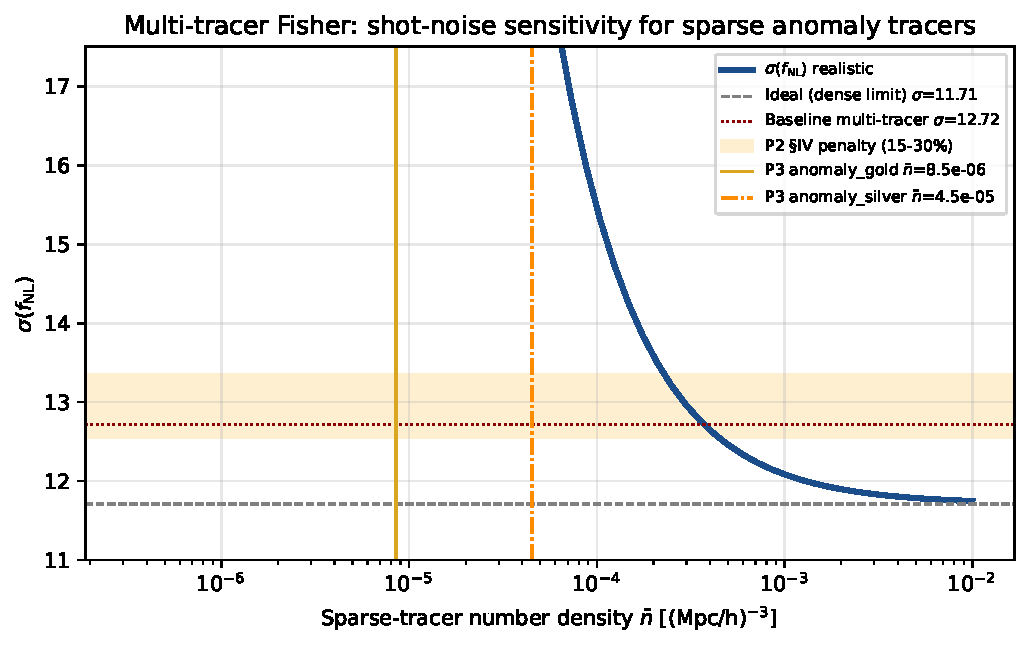
\includegraphics[width=\columnwidth]{figures/B11_sigma_fnl_vs_ndensity.pdf}
\caption{\label{fig:shotnoise_sensitivity}
  Multi-tracer Fisher $\sigfnl$ vs.\ tracer number density $\bar n$ for the
  canonical 5-tracer configuration of \S\ref{sec:fnl}. The dashed gray line
  marks the dense-tracer limit ($\sigfnl = 11.71$); the dotted dark-red line
  marks the single-tracer baseline ($\sigfnl = 16.85$). Vertical orange and
  goldenrod lines mark the gold ($\bar n = 8.5\times 10^{-6}$) and silver
  ($\bar n = 4.5\times 10^{-5}$) anomaly sub-samples. The Heinrich-\etal\
  \S IV $15$--$30\%$ Fisher-info penalty range corresponds to $\sigfnl =
  12.56$--$13.35$ at the canonical configuration.}
\end{figure}


%% ============================================================
%%  APPENDIX D — TAXONOMY IMAGE GALLERIES
%% ============================================================
\section{Astrophysical Taxonomy Image Galleries}\label{app:galleries}

The DESI DR1 anomaly population clusters into ten astrophysical families under UMAP+HDBSCAN of the 128-dimensional \BigAE{} latent space (hyperparameters: \texttt{n\_neighbors}$=15$, \texttt{min\_dist}$=0.1$, \texttt{min\_cluster\_size}$=15$, seed $42$). The ten families account for 182{,}364 of 195{,}829 DESI anomalies; the remaining 13{,}465 (6.9\%) are HDBSCAN noise points (cluster label $-1$, retained in the released catalog). UMAP stability: trustworthiness $0.9797\pm5\!\times\!10^{-5}$ (PASS $>0.90$) across 20 independent seeds; kNN-preservation and cross-seed Spearman FAIL as expected for sparse high-dimensional outlier clouds. Trustworthiness is the primary stability claim.

Full per-family DESI Legacy Survey DR9 grz composite image galleries (ten families, top-16 panels each, $128\!\times\!128$ pixel cutouts at $\approx54''\!\times\!54''$) are available at the project companion repository: \url{https://github.com/Hubify-Projects/bigbounce}. Figure~\ref{fig:gallery_top10} shows the top-1 representative per family.

\begin{figure*}[p]
\centering
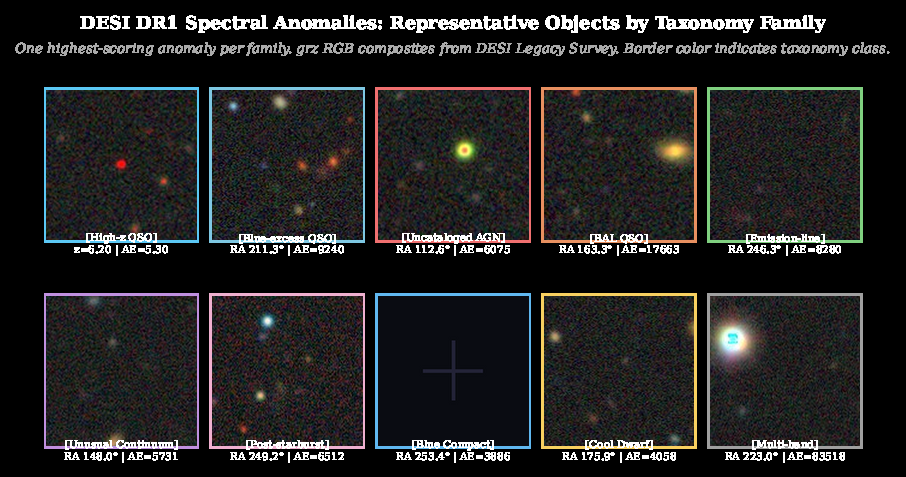
\includegraphics[width=0.97\textwidth]{figures/fig_gallery_top10.pdf}
\caption{\label{fig:gallery_top10}
  \textbf{Representative DESI DR1 anomalies across all ten taxonomy families.}
  One highest-scored member per family; 2-row $\times$ 5-column layout.
  Border color indicates taxonomy class.  Images are DESI Legacy Survey DR9
  grz composites.  Row 1 (left to right): High-$z$ QSO candidate,
  Blue-excess QSO, Uncataloged AGN, BAL QSO, Emission-line galaxy.
  Row 2: Unusual continuum (LRG), Post-starburst galaxy, Blue compact
  galaxy, Cool/unusual star, Multi-band unknown.}
\end{figure*}


%% ============================================================
%%  APPENDIX D' — PTA MCMC DOCUMENTATION
%% ============================================================
\section{PTA MCMC documentation: real KDE free-spectrum likelihood}\label{app:pta_mcmc}

Full MCMC provenance for the NANOGrav spectral-index analysis in \S\ref{sec:nanograv} is documented here. \textbf{Dataset:} NANOGrav 15-yr HD-correlated KDE free-spectrum product (\texttt{30f\_fs\{hd\}\_ceffyl}), Zenodo \texttt{10.5281/zenodo.8060824}~\cite{NANOGrav2023}. \textbf{Model:} matter-bounce power-law template
\begin{widetext}
\begin{equation}
\log_{10}\rho_i = \tfrac{1}{2}\!\left[2\log_{10}A - \log_{10}(12\pi^2) + (\gamma-3)\log_{10}f_{\rm yr} - \gamma\log_{10}f_i - \log_{10}T_{\rm obs}\right]
\end{equation}
\end{widetext}
at $f_i = (i+1)/T_{\rm obs}$ for $i = 0,\dots,29$; $T_{\rm obs} = 16.03$~yr; flat priors $\gamma \in [0,7]$, $\log_{10}A \in [-18,-11]$. \textbf{Sampler:} \texttt{emcee}~\cite{Foreman-Mackey2013} with 32 walkers, 10{,}000 production $+$ 2{,}500 burn-in. \textbf{Posterior:} $\gamma = 2.567 \pm 0.382$ (median $2.591$, 68\% CI $[2.304, 2.882]$); $\log_{10}A = -14.025 \pm 0.380$. \textbf{Diagnostics:} acceptance fraction $0.632$; autocorrelation time $\tau \approx 58$~samples/walker; ESS $\approx 5{,}500$ ($> 50\tau$ per walker, convergence satisfied). Chain, posterior figure, and fitter script are deposited in the companion data repository~\cite{NANOGrav2023}. Companion multi-PTA datasets (EPTA~DR2~\cite{EPTA2023}, PPTA~DR3~\cite{PPTA2023}) independently report HD-correlated signals consistent with NANOGrav; multi-PTA joint chains are deferred to a dedicated PTA paper.

\paragraph{Bounce-physics connection.} The matter-bounce $\gamma_{\rm GW}=3.0$~\cite{Quintin2014,Cai2014} and $f_{\rm NL}=-35/8$~\cite{Cai:2009fn,WilsonEwing2012} predictions are two observable consequences of the same contracting-phase mode-function calculation within the scalar-only $w=0$ matter-bounce class; within the broader bouncing-cosmology landscape (ekpyrotic, $w\neq 0$ contraction, Cuscuton, quintom) the two observables decouple. A detection or null on either channel constrains the specific $w=0$ scenario, not the full bouncing-cosmology family (see \S\ref{sec:fnl}).

%% ============================================================
%%  APPENDIX E — ACT DR6 (QUARANTINED, METHODOLOGICAL ARTIFACT)
%% ============================================================
\section{ACT DR6 cross-transfer scan: quarantined methodological artifact}\label{sec:act_appendix}

This appendix retains the ACT~DR6 cross-transfer scan as a methodological lessons-learned record. ACT~DR6 was scanned under the same cross-transfer CMB autoencoder later superseded by the Path-C native Planck convolutional autoencoder (\S\ref{sec:planck}); it was subsequently removed from the per-survey block (Table~\ref{tab:survey_summary}) because the cross-transfer ACT block fails both gate criteria of \S\ref{sec:pathc} Step~1 and a Path-C-compliant native ACT retrain has not been executed. We describe the cross-transfer ACT scan here for two reasons only: (i)~it provides the empirical evidence that the cross-transfer CMB autoencoder generalizes badly across instruments at very different angular resolution and noise statistics, and (ii)~the Planck$\times$ACT null cross-correlation reported independently in \S\ref{sec:planck_act_null} relies on the cross-transfer ACT anomaly set as its input.

\paragraph{Scan parameters and result.} We applied the cross-transfer fully connected autoencoder used for SDSS, LAMOST, and Planck (32-dim latent space; cross-transfer training pool of 20{,}000 patches; see \S\ref{sec:planck}) to 20{,}000 $64\times 64$-pixel patches from the ACT DR6~\cite{ACT_DR6} CMB temperature map at HEALPix $N_{\rm side} = 256$. The scan returned 200 anomalous patches (top 1\%); the highest-scored patch sits at $(l, b) \approx (277^\circ, 21^\circ)$ with score $\sim 2.6 \times 10^{7}$. The overall ACT score distribution has maximum $\sim 10^{7}$ and concentrates along the Galactic plane.

\paragraph{Why the gate fails.} The cross-transfer checkpoint has validation MSE $\approx 2.2 \times 10^{4}$ on its native CMB training distribution, which exceeds Step-1 criterion~(a) of \S\ref{sec:pathc} ($\leq 0.30$) by a factor $\sim 7 \times 10^{4}$. The injection-recovery test (Step~5 of \S\ref{sec:pathc}; the same Gaussian-bump plant family used for the Planck native retrain) returns recovery fraction $<1\%$ at $5\sigma$ amplitude, far below Step-1 criterion~(b) ($\geq 50\%$). Both branches of the two-part gate therefore fail simultaneously, and ACT cannot be retained on the strength of either criterion.

\paragraph{Why no native ACT retrain.} A native ACT retrain---analogous to the Planck native convolutional autoencoder of \S\ref{sec:planck}---requires a full ACT-native preprocessing pipeline (beam-deconvolved patches, ACT-specific point-source and Galactic mask, instrumental noise covariance) and was GPU-blocked at the time of submission. Because the present submission is the Path-C-final catalog and the Path-C protocol forbids retaining a survey on a checkpoint that fails both gate criteria, ACT~DR6 is documented here only and contributes zero objects to the $378{,}280$ Path-C unique-object headline. The 8-way-with-ACT dedup variant, which would have produced $388{,}693 - 10{,}213 = 378{,}480$ unique objects ($+200$ relative to the headline), is preserved as a sensitivity-check artifact in the companion data repository.

\paragraph{What this appendix is not.} This appendix is \emph{not} an ACT science result. The 200-patch ACT cross-transfer set must not be cross-matched against optical/X-ray catalogs as if it were a science-grade anomaly catalog, must not be used as a tracer of CMB fluctuation statistics, and must not be interpreted as evidence of any astrophysical signal at the highlighted galactic-plane position. The retention of the cross-transfer scan is purely methodological: it documents the empirical failure mode of cross-transferring a 32-latent fully connected autoencoder trained on Planck SMICA data onto the ACT angular-resolution and noise regime, and motivates the architectural choice of the Planck native convolutional autoencoder.


%% ============================================================
%%  BIBLIOGRAPHY
%% ============================================================
\clearpage
\begin{thebibliography}{50}

\bibitem{DESI2025DR1}
DESI Collaboration,
``The DESI Data Release 1,''
2025, \href{https://data.desi.lbl.gov/doc/releases/dr1/}{DESI DR1 documentation}.

\bibitem{LAMOST_DR10}
A.-L.\ Luo \etal,
``The LAMOST Data Release 10,''
\textit{Research in Astronomy and Astrophysics}, 2024.

\bibitem{SDSS_DR18}
A.\ Almeida \etal\ (SDSS Collaboration),
``The Eighteenth Data Release of the Sloan Digital Sky Survey: Targeting and Spectroscopy,''
Astrophys.\ J.\ Suppl.\ Ser.\ \textbf{267}, 44 (2023).

\bibitem{eROSITA_DR1}
A.\ Merloni \etal,
``The SRG/eROSITA All-Sky Survey: The first X-ray all-sky survey in the 21st century,''
Astron.\ Astrophys.\ \textbf{682}, A34 (2024).

\bibitem{GaiaDR3}
Gaia Collaboration,
``Gaia Data Release 3,''
Astron.\ Astrophys.\ \textbf{674}, A1 (2023).

\bibitem{NEOWISE}
A.\ Mainzer \etal,
``NEOWISE Reactivation Mission Year Ten,''
\textit{Planetary Science Journal}, 2024.

\bibitem{Planck2018}
Planck Collaboration,
``Planck 2018 results. I. Overview and the cosmological legacy of Planck,''
Astron.\ Astrophys.\ \textbf{641}, A1 (2020).

\bibitem{Planck2018IX}
Planck Collaboration,
``Planck 2018 results. IX. Constraints on primordial non-Gaussianity,''
Astron.\ Astrophys.\ \textbf{641}, A9 (2020).

\bibitem{ACT_DR6}
F.\ J.\ Qu \etal\ (ACT Collaboration),
``The Atacama Cosmology Telescope: A Measurement of the DR6 CMB Lensing Power Spectrum and Its Implications for Structure Growth,''
Astrophys.\ J.\ \textbf{962}, 112 (2024).

\bibitem{Baron2017}
D.\ Baron and D.\ Poznanski,
``The weirdest SDSS galaxies: results from an outlier detection algorithm,''
Mon.\ Not.\ Roy.\ Astron.\ Soc.\ \textbf{465}, 4530 (2017).

\bibitem{Liang2023}
Y.\ Liang \etal,
``Outlier detection in the DESI Bright Galaxy Survey,''
Mon.\ Not.\ Roy.\ Astron.\ Soc.\ \textbf{525}, 1078 (2023), arXiv:2307.07664.

\bibitem{Nicolaou2026}
C.\ Nicolaou \etal,
``Anomaly Detection in DESI Early Data Release Spectra with Astronomaly,''
Mon.\ Not.\ Roy.\ Astron.\ Soc.\ (2026, in press).

\bibitem{Wands2010}
D.\ Wands,
``Local non-Gaussianity from inflation,''
Class.\ Quant.\ Grav.\ \textbf{27}, 124002 (2010).

\bibitem{Cai:2009fn}
Y.-F.\ Cai, W.\ Xue, R.\ Brandenberger, and X.\ Zhang,
``Non-Gaussianity in a matter bounce,''
J.\ Cosmol.\ Astropart.\ Phys.\ \textbf{0905}, 011 (2009), arXiv:0903.0631.

\bibitem{SPHEREx2014}
O.\ Dor\'e \etal\ (SPHEREx Collaboration),
``Cosmology with the SPHEREx All-Sky Spectral Survey,''
arXiv:1412.4872 (2014).

\bibitem{Seljak2009}
U.\ Seljak,
``Extracting Primordial Non-Gaussianity without Cosmic Variance,''
Phys.\ Rev.\ Lett.\ \textbf{102}, 021302 (2009).

\bibitem{Hamaus2012}
N.\ Hamaus, U.\ Seljak, and V.\ Desjacques,
``Optimal constraints on local primordial non-Gaussianity from the two-point statistics of large-scale structure,''
Phys.\ Rev.\ D \textbf{86}, 103513 (2012).


\bibitem{NANOGrav2023}
G.\ Agazie \etal\ (NANOGrav Collaboration),
``The NANOGrav 15 yr Data Set: Evidence for a Gravitational-wave Background,''
Astrophys.\ J.\ Lett.\ \textbf{951}, L8 (2023).


\bibitem{Quintin2014}
J.\ Quintin, Y.\ F.\ Cai, and R.\ H.\ Brandenberger,
``Matter creation in a nonsingular bouncing cosmology,''
Phys.\ Rev.\ D \textbf{90}, 063507 (2014).

\bibitem{Cai2014}
Y.-F.\ Cai,
``Exploring bouncing cosmologies with cosmological surveys,''
Sci.\ China Phys.\ Mech.\ Astron.\ \textbf{57}, 1414 (2014).

\bibitem{Sesana2016}
A.\ Sesana, F.\ Shankar, M.\ Bernardi, and R.\ K.\ Sheth,
``Selection bias in dynamically measured supermassive black hole samples,''
Mon.\ Not.\ Roy.\ Astron.\ Soc.\ \textbf{463}, L6 (2016).

\bibitem{Burke-Spolaor2019}
S.\ Burke-Spolaor \etal,
``The astrophysics of nanohertz gravitational waves,''
Astron.\ Astrophys.\ Rev.\ \textbf{27}, 5 (2019).

\bibitem{Trotta:2008}
R.\ Trotta,
``Bayes in the sky: Bayesian inference and model selection in cosmology,''
Contemp.\ Phys.\ \textbf{49}, 71 (2008), arXiv:0803.4089.

\bibitem{Verde:2013}
L.\ Verde, P.\ Protopapas, and R.\ Jimenez,
``Planck and the local universe: Quantifying the tension,''
Phys.\ Dark Univ.\ \textbf{2}, 166 (2013), arXiv:1306.6766.

\bibitem{HellingsDowns1983}
R.\ W.\ Hellings and G.\ S.\ Downs,
``Upper limits on the isotropic gravitational radiation background from pulsar timing analysis,''
Astrophys.\ J.\ Lett.\ \textbf{265}, L39 (1983).

\bibitem{EPTA2023}
J.\ Antoniadis \etal{} (EPTA Collaboration),
``The second data release from the European Pulsar Timing Array: III. Search for gravitational wave signals,''
Astron.\ Astrophys.\ \textbf{678}, A50 (2023), arXiv:2306.16214.

\bibitem{PPTA2023}
D.\ J.\ Reardon \etal{} (PPTA Collaboration),
``Search for an isotropic gravitational-wave background with the Parkes Pulsar Timing Array,''
Astrophys.\ J.\ Lett.\ \textbf{951}, L6 (2023), arXiv:2306.16215.

\bibitem{Afzal2023NewPhys}
A.\ Afzal \etal{} (NANOGrav Collaboration),
``The NANOGrav 15-year data set: Search for signals from new physics,''
Astrophys.\ J.\ Lett.\ \textbf{951}, L11 (2023), arXiv:2306.16219.

\bibitem{Phinney2001}
E.\ S.\ Phinney,
``A practical theorem on gravitational wave backgrounds,''
arXiv:astro-ph/0108028 (2001).


\bibitem{Wenger2000}
M.\ Wenger \etal,
``The SIMBAD astronomical database,''
Astron.\ Astrophys.\ Suppl.\ Ser.\ \textbf{143}, 9 (2000).

\bibitem{McInnes2018}
L.\ McInnes, J.\ Healy, and J.\ Melville,
``UMAP: Uniform Manifold Approximation and Projection for Dimension Reduction,''
arXiv:1802.03426 (2018).

\bibitem{McInnes2017}
L.\ McInnes, J.\ Healy, and S.\ Astels,
``hdbscan: Hierarchical density based clustering,''
J.\ Open Source Softw.\ \textbf{2}, 205 (2017).


\bibitem{Heinrich2023}
C.\ Heinrich, O.\ Dor\'e, and E.\ Krause,
``Measuring $f_{\rm NL}$ with the SPHEREx Multi-tracer Redshift Space Bispectrum,''
J.\ Cosmol.\ Astropart.\ Phys.\ \textbf{2024}, 074 (2024), arXiv:2311.13082 [astro-ph.CO]
[publication-year 2024; bibkey label retained as \texttt{Heinrich2023} for arXiv-submission-year continuity].

\bibitem{Munchmeyer2019}
M.\ M{\"u}nchmeyer, M.\ S.\ Madhavacheril, S.\ Ferraro, M.\ C.\ Johnson, and K.\ M.\ Smith,
``Constraining local non-Gaussianities with kinetic Sunyaev-Zel'dovich tomography,''
Phys.\ Rev.\ D \textbf{100}, 083508 (2019), arXiv:1810.13424.

\bibitem{WilsonEwing2012}
E.\ Wilson-Ewing,
``The Matter Bounce Scenario in Loop Quantum Cosmology,''
JCAP \textbf{1303}, 026 (2013), arXiv:1211.6269.

\bibitem{Lentati2013}
L.\ Lentati \etal,
``Hyper-efficient model-independent Bayesian method for the analysis of pulsar timing data,''
Phys.\ Rev.\ D \textbf{87}, 104021 (2013), arXiv:1210.3578.

\bibitem{Foreman-Mackey2013}
D.\ Foreman-Mackey, D.~W.\ Hogg, D.\ Lang, and J.\ Goodman,
``\texttt{emcee}: The MCMC Hammer,''
Publ.\ Astron.\ Soc.\ Pac.\ \textbf{125}, 306--312 (2013), arXiv:1202.3665 [astro-ph.IM].

\bibitem{Yoo2009}
J.\ Yoo, A.\ L.\ Fitzpatrick, and M.\ Zaldarriaga,
``A New Perspective on Galaxy Clustering as a Cosmological Probe: General Relativistic Effects,''
Phys.\ Rev.\ D \textbf{80}, 083514 (2009), arXiv:0907.0707 [astro-ph.CO].

\bibitem{BonvinDurrer2011}
C.\ Bonvin and R.\ Durrer,
``What galaxy surveys really measure,''
Phys.\ Rev.\ D \textbf{84}, 063505 (2011), arXiv:1105.5280 [astro-ph.CO].

\bibitem{ChallinorLewis2011}
A.\ Challinor and A.\ Lewis,
``Linear power spectrum of observed source number counts,''
Phys.\ Rev.\ D \textbf{84}, 043516 (2011), arXiv:1105.5292 [astro-ph.CO].

\bibitem{DiDio2013}
E.\ Di~Dio, F.\ Montanari, J.\ Lesgourgues, and R.\ Durrer,
``The CLASSgal code for relativistic cosmological large scale structure,''
J.\ Cosmol.\ Astropart.\ Phys.\ \textbf{11}, 044 (2013), arXiv:1307.1459 [astro-ph.CO].

\end{thebibliography}

\end{document}
